\documentclass[a4paper, openany]{memoir}

\usepackage[utf8]{inputenc}
\usepackage[T1]{fontenc} 
\usepackage[english]{babel}

\usepackage{fancyhdr}
\usepackage{float}

\usepackage{amsmath}
\usepackage{amsthm}
\usepackage{amssymb}
\usepackage{enumitem}
\usepackage{multicol}
\usepackage[bookmarksopen=true,bookmarksopenlevel=2]{hyperref}
\usepackage{tikz}
\usepackage{indentfirst}

\usepackage{listings}
\usepackage{xcolor}

\pagestyle{fancy}
\fancyhf{}
\fancyhead[LE]{\leftmark}
\fancyhead[RO]{\rightmark}
\fancyhead[RE, LO]{WAD}
\fancyfoot[LE, RO]{\thepage}
\fancyfoot[RE, LO]{Pete Gautam}

\definecolor{ocre}{RGB}{52,177,201}
\definecolor{ultramarine}{RGB}{0,45,97}
\definecolor{mybluei}{RGB}{0,0,255}
\definecolor{myblueii}{RGB}{100,0,100}
\definecolor{myblueiii}{RGB}{50,234,253}

\definecolor{codegreen}{rgb}{0,0.6,0}
\definecolor{codegray}{rgb}{0.5,0.5,0.5}
\definecolor{codepurple}{rgb}{0.58,0,0.82}
\definecolor{backcolour}{rgb}{0.95,0.95,0.92}

\lstdefinestyle{mystyle}{
    backgroundcolor=\color{backcolour},   
    commentstyle=\color{codegreen},
    keywordstyle=\color{blue},
    numberstyle=\tiny\color{codegray},
    stringstyle=\color{codepurple},
    basicstyle=\ttfamily\footnotesize,
    breakatwhitespace=false,         
    breaklines=true,                 
    captionpos=b,                    
    keepspaces=true,                 
    numbers=left,                    
    numbersep=5pt,                  
    showspaces=false,                
    showstringspaces=false,
    showtabs=false,                  
    tabsize=2
}
\lstset{style=mystyle}


\lstdefinelanguage{XML}{
    sensitive=false, 
    keywords={
        xml, breakfast_menu, food, name, price, calories,
        DOCTYPE, ELEMENT, note, to, from, heading, body,
        xs, complexType, sequence, type,
        employees, employee, firstName, lastName,
    },  
    ndkeywords={},  
    morecomment=[s]{<!--}{-->},
    stringstyle=\color{purple}\ttfamily,
    morestring=[b]',
    morestring=[b]"
}

\lstdefinelanguage{JavaScript}{
  keywords={typeof, new, true, false, catch, function, return, null, try, catch, finally, switch, var, if, in, while, do, else, case, break, document, class, this, export, boolean, throw, implements, import},
  keywordstyle=\color{blue}\bfseries,
  ndkeywords={},
  ndkeywordstyle=\color{darkgray}\bfseries,
  identifierstyle=\color{black},
  sensitive=false,
  comment=[l]{//},
  morecomment=[s]{/*}{*/},
  commentstyle=\color{purple}\ttfamily,
  stringstyle=\color{red}\ttfamily,
  morestring=[b]',
  morestring=[b]"
}

\renewcommand{\headrulewidth}{1.5pt}

\chapterstyle{thatcher}
\setcounter{chapter}{2}

\begin{document}
\chapter{Other Aspects of Web Development}

\section{Complexities in web development}
There are many complexities in web development. The structure and the nature of the application is one of the reasons. The issues in this section are: 
\begin{itemize}
    \item the hypertext structure of the website- there can be a lot of content present spread out throughout the website, with links connecting them. They can be in different servers or different (human) languages and need to be connected to each other; 
    \item the presentation and the layout- the content should be presented in an asthetic fashion; 
    \item content usage and management- there might be a lot of content, e.g. Amazon or Netflix, and it is a huge challenge to make everything accessible, timely and up to date; and
    \item the overall service usage of the site.
\end{itemize}
Another issue is the usage of the application. The issue in this section are:
\begin{itemize}
    \item the users expect instant online access- we cannot show the result of some query that a user has performed after a minute because they expect it to be instantaneous;
    \item the users expect the content to be available permanently- we cannot have long website downtime; 
    \item a wide variety of usually anonymous users, meaning that we aren't sure who we are designing the content for, their level of expertise is or their cultural backgrounds; and
    \item users make use of a variety of devices to access the website, from small phones to large laptops.
\end{itemize}
The final issue is the development process behind the application. The issues here are:
\begin{itemize}
    \item the development by a multidisciplinary team with experts and novices- the team has people with different experience and work out how to produce the site;
    \item the state of continuous development- after the site is released, we still need to manage them and constantly fixing bugs, scaling, adding new features, and so on; and
    \item a mixture of legacy technologies and immature technologies- some technology might be old while others might be brand new and have some bugs.
\end{itemize}

\subsection{Structure and Nature}
The hypertext structure means that there is a need to:
\begin{itemize}
    \item avoid user disorientation and cognitive overload;
    \item provide multiple paths to support users with different requirements; and
    \item provide a good superstructure, including search facilities, site map and guided tours.
\end{itemize}
The presentation or user interface must be:
\begin{itemize}
    \item self-explanatory with no user manuals for the site;
    \item aesthetically pleasing and adaptable to different contexts- ideally self-ad-apting, but somehow there must be a version of the user interface which works in each context.
\end{itemize}
The content delivery must be:
\begin{itemize}
    \item fast, up-to-date, consistent and reliable;
    \item secure- particularly for financial transactions;
    \item adaptable to different contexts in terms of how much can be delivered.
\end{itemize}

\subsection{Users and Usage}
Users expect immediate and fast availability. They also expect permanent availability. They also expect access on a variety of devices- the quality of service becomes an issue. They have a very diverse background culturally and linguistically. They have a low tolerance threshold for slow or hard-to-use sites. There may be a lot of users accessing the site.

\subsection{Development Process}
One of the main issues in the development process is the nature of the developers. In particular:
\begin{itemize}
    \item Professional development is by a multidisciplinary team. It is made up of programmers, graphic designers and domain experts;
    \item Much development is by amateurs or inexperienced programmers;
    \item Development can be communal by a geographically distributed group.
\end{itemize}
The development environment consists of issues as well. For example,
\begin{itemize}
    \item There are a wide variety of technologies, each programmed differently;
    \item Many of the technologies are immature, but some are legacy;
    \item Each of the technologies has multiple competing products, and upgrading the site often means changing the product.
\end{itemize}
The development process itself also has issues, such as:
\begin{itemize}
    \item There is no set of accepted internet application development methodologies;
    \item The process must be flexible, but not rigid;
    \item Parallel development of components (and even versions) is necessary;
    \item Agile processes seem valuable here.
\end{itemize}

\subsection{Types of web applications}
There are many types of web applications, including:
\begin{itemize}
    \item Static websites- originally, web applications were just collections of hand-built HTML pages. These required manual update and introduced the possibility of inconsistency;
    \item Interactive websites- forms, selective menus and radio buttons on web pages offer the possibility of selectively chosen pages generated by server-side programs. CGI was the first technology, but it has been superseded by others (ASP, ISP, PHP, Cold Fusion, etc.)
    \item Transactional websites- forms also offer the capture of data and database storage at the server. However, the data management may be separated from the internet server.
    \item Workflow-based websites- support for functionality is expressed as a sequence of pages, reflecting a business process, like booking a flight.
    \item Portal-oriented websites- one point of access is given to multiple websites, e.g. virtual shopping malls.
    \item Collaborative websites- web sites which permit multiple users sharing information management, e.g. wikis such as wikipedia.
    \item Social websites- a focal point for communities, e.g. photo-sharing sites, facebook, etc.
    \item Mobile and ubiquitous sites- ``web'' applications increasingly provide access by small, mobile and non-visual devices (i.e. phones) as well as data capture by sensors.
\end{itemize}
\newpage

\section{System Architecture}
Every component of a system must be designed. The architecture of the system shows the blueprint or plans of how each component fits together. Architectural diagrams can be at various levels: data structure/algorithm/object level; component/library level; or application level. Various diagrams are needed. Here, we focus on the application or the high level system architecture.


\subsection{Tiered Architectures}
\noindent The main task that any application must support is:
\begin{itemize}
    \item user interface management;
    \item the implementation of algorithms, e.g. the business logic;
    \item the information manipulation; and
    \item the data storage.
\end{itemize}
A monolitic program in Java does all of the following:
\begin{itemize}
    \item user interface, with Swing or JavaFX;
    \item algorithms, in methods;
    \item information manipulation in methods, e.g. sort methods;
    \item data storage, using File I/O.
\end{itemize}
A single tier architecture can be represented as follows:
\begin{center}
    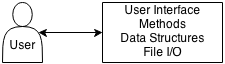
\includegraphics[scale=0.8]{src/L7I1.png}
\end{center}
Here, we have one user interacting with the system. An example of this would be running an application in the PC. It is very easy to design, but is not scalable- it does not separate out the concerns and is not part of a network.

\noindent The structure of applications have changed from monolithic programs as single unit in which every aspect of the application is coded to tiered system in which different aspects are separated into different levels.

\noindent The advantage of the tiered architectures are:
\begin{itemize}
    \item each tier can be coded separately without one programmer having to deal with everything; and
    \item the different tiers can be distributed over the network, leading to increasing efficiency.
\end{itemize}
\noindent But, the tiers must interact effectively. There must be well-defined interface between adjacent tiers. Internet protocols and database connection software do this as well.

\subsubsection{Two-tier architectures}
A two-tier architecture supplies a basic network between the client and the serv-er. The web model is a two-tier architecture- the web browser is running on the client's device. It makes a request to the web server, and it gets back a response, which is a webpage. This improves scalability, divides the user interface from the data layers.

\noindent In a two-tier architecture, one of the most important things is to manage data and information. Data and information management is common in many applications. Below are few of the common functionalities:
\begin{itemize}
    \item Handling and dealing with large amounts of data;
    \item Accessing a share repository of data, which is highly beneficial to facilitate information flows between actors;
    \item Storing, retrieving, modify, securing;
\end{itemize}
Database systems and information retrieval systems provide ways to manage this data and information (efficiently).

\noindent It is difficult and time-consuming to write the code which accesses large amou-nts of data efficiently. Instead, we separate the concerns. We let a database system handle the data management, and then use a client application to interact with the database. The client acts like a database user, sending in queries and updates and making use of the result. A simple way of doing this is by coding SQL statements as string inside the program.

\noindent The following is a revised 2-tier diagram:
\begin{center}
    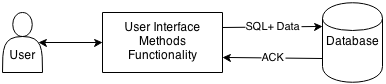
\includegraphics[scale=0.8]{src/L7I2.png}
\end{center}
This is a fat client model. It is the standard architecture for getting an application (e.g. Java-based) to work on top of a database.

\noindent There are issues with the 2-tier architecture. The application with a 2-tier architecture only distinguish between client and server process. The client processes are those controlling the logic of the application and the user interface. On the other hand, the server processes are those that supply resources (e.g. data) to the clients. However, this puts a lot of the load on the client. It also might tie the client software to the database software, so changes in one affect the other.

\noindent A static web application consists of a set of hyper-linked HTML files. Each HTML file describes one page of the web site. Each page includes one or more links to other pages. If a user clicks a link or enters a URL, then a request is sent to the web server, identifying the next page to load.

\noindent A static web-application uses a thin client model. The following is a thin client model 2-tier diagram:
\begin{center}
    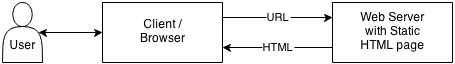
\includegraphics[scale=0.8]{src/L7I3.png}
\end{center}
This is the standard architecture serving up static content on the web. This is a simpler setup than the previous system.

\noindent We can start to complicate things by considering CSS. Initially, the HTML files contained all the information on how to render the page- the text/data (html), along with the style (css). With lots of pages, there is lots of overhead in creating and maintaining the site. So, we should separate the concerns. We should use external CSS which act upon the different elements in the HTML. The web server/application returns an HTML file and a CSS file, i.e. one to hold the content, and one to represent the style. This is an extended thin client.

\noindent The extended thin client has the following 2-tier diagram:
\begin{center}
    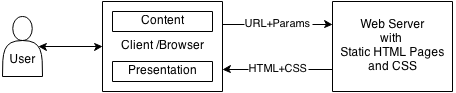
\includegraphics[scale=0.8]{src/L7I4.png}
\end{center}
The layers within the client tier handle the content and the look/feel. The content layer represents/stores the data. The presentation layer renders the data.

\noindent On a site, many pages will have similar structure, and a lot of repeated content, i.e. headers, footers, navigation, etc. We use a template and decompose repeated element, i.e. separate the concerns. It is better to have a program which generates pages by merging a template with the specific page data. The appropriate data depends on the URL and the parameters in the URL. This enables the provision of dynamic content, but requires a more sophisticated architecture.

\noindent Anywhere, anytime, anyplace we see repeated code, we should refactor. We should look through methods, objects, templates and applications. We should aim to extract the common parts; parametrise the parts that change; create a template; and write a program to use the template given a set of parameters.

\noindent Now, we introduce user interaction. Clicking a link only provides the link information. Forms take input, but we need to understand what happens when we hit the submit button. This enables the provision of interaction, but this requires the server-side program to be able to deal with the data from the form. HTTP provides methods for sending the data entered by the user to the program by GET and POST commands. The GET command is to request and receive information, while POST is to submit data from the web browser.

\noindent This extra functionality is depicted as the extended thin client and extended server. It has the following architecture diagram:
\begin{center}
    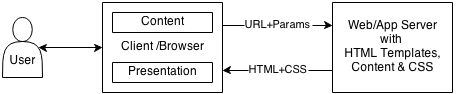
\includegraphics[scale=0.8]{src/L7I5.png}
\end{center}
The layers within the client tier handle the content and the look/feel. The server now houses a web server and an application server. The web server handles incoming requests and sends outgoing responses. It routes them to/from the correct application server. The application server is typically a script that dynamically generates a response given a request.

\subsubsection{Three to N-tier architectures}
An improvement to 2-tier architecture is to separate the application into three (or N-) tiers. These tiers are:
\begin{itemize}
    \item presentation processes- these deal exclusively with the user interface. For instance, this might be through the use of a browser or other user agent;
    \item application processes- these deal with the logic of the application, queries, calculations, etc. There is either one (3-tier) or more (N-tier) of such processes; and
    \item data source processes- these supply the data from a database (binary) or a file (e.g. XML).
\end{itemize}
The following is a basic 3-tier architecture:
\begin{center}
    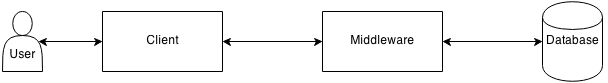
\includegraphics[scale=0.8]{src/L8I1.png}
\end{center}
Here, the client handles the interaction with the user; the middleware handles the application logic; and the database stores the data. The database persists and manages the data associated with the application. This architecture further separates out responsibilities (presentation, logic and data).

\noindent Within the middleware tier, usually there is a webserver, an application server, and potential media servers. The webserver handles incoming requests, directing them to the appropriate server. The servers could be on the same machine or different machines. An N-tier architecture makes the website more scalable.

\noindent The following is an N-tier architecture:
\begin{center}
    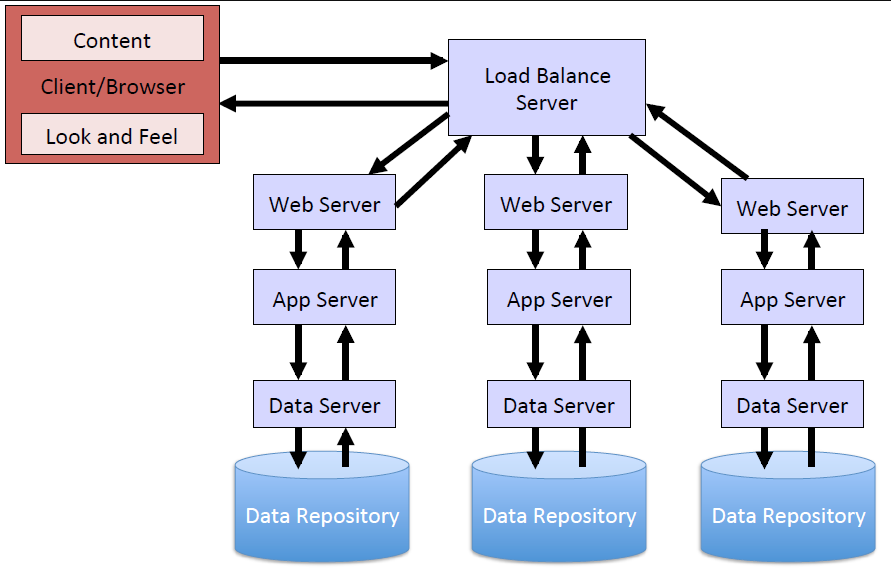
\includegraphics[scale=0.5]{src/L8I2.PNG}
\end{center}
Here, we have a load balance server, along with the web, app and data server, connected to a data repository. If there are many users trying to access the content at once, they are hitting the load-balance server, which decides to which parallel setup we can redirect the traffic to.

\noindent There are two ways to balance the load:
\begin{itemize}
    \item Using a domain name server such that when a URL is resolved, it rotates through a series of IP addresses that route the message to that machine;
    \item Using a load-balancing server, which farms out the request to available machines. Machine in the farm inform the load-balancing server of their load so that the load can be balanced.
\end{itemize}

\noindent In summary, tiers enable the separation of concerns. They help encapsulate complexity- they can be broken down into layers or into sub-tiers. Tiers can be distributed across a number of machine. This provides flexibility and more security (as clients do not interact directly with the database). Tiers can be replicated across a number of machines. This provides scalability.

\subsection{Top down and bottom up design}
We have seen many system architecture diagrams. They are integral to illustrate the ideas and the designs clearly. In general, there are two types of such designs- top down design and bottom up design.

\noindent The designs we have seen until now has been top-down design. Starting from a high-level design is useful because:
\begin{itemize}
    \item it helps describe the system at a level which makes the goals, scope and responsibilities clear;
    \item the abstraction provides a tool for communicating the design;
    \item it permits the specific technologies to be chosen later or to be changed;
    \item we have better maintenance, more reusability, and higher profit.
\end{itemize}
On the other hand, the bottom-up design is about piecing together components to give rise to more complex systems. Thus, it makes the original element sub-system of the emergent system. The most specific and basis individual components of the system are first developed. These elements are then linked together to form larger subsystems, which then in turn are linked, sometimes in many levels, until a complete top-level system is formed. This strategy often resembles a ``seed'' model, by which the beginnings are small but eventually grow in complexity and completeness.

\noindent There are some advantages and disadvantages when using top-down design. Top-down separates the low-level work from the higher-level abstractions. This can lead to a modular design. The development can therefore be self-contained (i.e. tiered). It emphasises planning and system understanding. However, coding is late, and testing even later. Skeleton code can show how everything integrates.

\noindent Similarly, there are some advantages and disadvantages when using bottom-up design. Coding begins early, and testing can be performed early as well. On the other hand, it requires really good intuitions to determine the functionality of modules. low-level design decisions can have major impact on solutions. It risks integration problems- how do the components link together. It is often used to add a new module to an existing system.

\noindent Architects need to communicate to developers how the application and its components fit together and who is responsible for what. The designs also serve as a communication tool with the client. It is important to be able to draw and read such diagrams, especially when projects become large and complex.

\subsection{Notation for System Architecture}
The modified dataflow language has many entities such as user, client and middleware. There is a notation for each one of them, and we will go through them individually below.

\noindent The user or customer instigates and interacts with the services or the applications provided. There are various types of users, such as end users (of varying abilities), administrators, developers, other systems and so on.

\noindent The client and the interface presented takes on many forms, and vary greatly. It can be a web browser on a PC, tablet, mobile, etc. It could also be an API for other systems, agents, developers, etc. It might be devices and robots, or even sensors.

\noindent The middleware houses an array of possible components from:
\begin{itemize}
    \item domain name servers;
    \item load balancing servers;
    \item web servers;
    \item application servers;
    \item caching servers.
\end{itemize}
Typically, the first three are predefined or configured using a standard software. The application server is what is mainly of interest, i.e. what needs to be developed. Often, we represent it as a single component that brokers requests between the client and the database even though it encapsulates a number of other components.

\noindent A database server is usually employed to handle the data management side of applications, i.e. Postgres, SQLServer and MySQL. While the system is already in existence, it needs to be configured, i.e. the database tables have to be define and populated. To specify this part more precisely, ER diagrams can be used.

\noindent The logs represent data sinks. The application outputs data, but does not read it back directly. 

\noindent External services represent applications and services that are used by the application. They provide an API or interface of some kind that can be used to interact with the service.

\noindent For each box, we could choose to specify the technology/device used, e.g.:
\begin{itemize}
    \item The client is a web browser on a mobile device, using HTML, CSS and JS;
    \item The middleware is the Apache web server, with an application server built using Django;
    \item The database is the MySQL database server.
\end{itemize}

\noindent Arrows are used to denote the flow of information. The direction of the arrow denotes the direction of the communication. Most communication are both ways, i.e. a request is made and that is followed by a response. This shows how the entities are related.
\newpage

\section{Information Architecture}
Information architecture is concerned with structuring and categorising information to help navigation and usefulness of the product along with manageability of the information. This is about creating an environment for users and clients to interact with the system in such a way that it is meeting all their needs.

\noindent We will look at the structural design of shared environments. This is a combination of organisation, labelling, search and navigation systems within web sites and intranets. We find that it is an art and a science of shaping information products and experiences to support usability and findability. It is an emerging discipline and community of practice, focused on bringing principles of design and architecture to the digital landscape.

\noindent To be successful as information  architects, we need to think like a user. Therefore, we need to understand the potential for a gap between the user and the organisation- the communication chasm. Users have particular needs, goals, aims and objects. The key problem is to figure out whether the organisation is providing answers, suggestions, solutions, options, etc.

\noindent Users have information needs. There are a lot of audience types. We need to understand the scope and the volume of the content, how it is structured, and its metadata. All of this occurs within the content of a business operation. The business has a strategy, and finite amount of resources, culture and politics atmosphere associated with it, including the workflow.

\noindent To make these systems of information, we need to understand the interdependent nature of users, content and context. The following is called the information ecology:
\begin{center}
    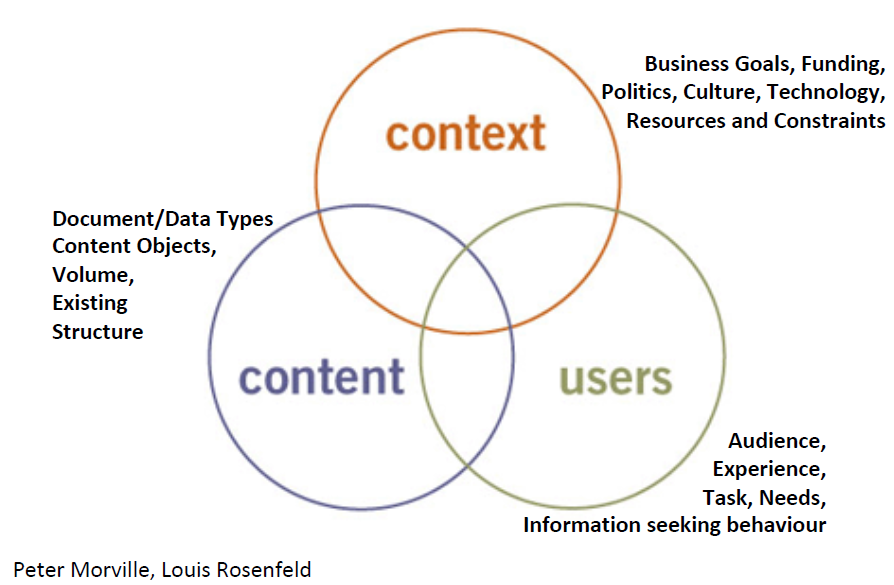
\includegraphics[scale=0.6]{src/L8I3.PNG}
\end{center}

\noindent Information architecture is important because it makes us consider the user. There is a cost of finding information- time is lost, and people get frustrated. Even worse, if the information is not found, the user may make a bad decision or find a different service. There is also cost of construction- staffing, technology, planning, and finding bugs. Moreover, there is cost of maintenance- we must always manage the content and redesign in future as appropriate. There is a cost of training the employees. Moreover, the value of brand can be severely affected by a bad product.

\noindent We can talk about information architecture in terms of the following three concepts:
\begin{itemize}
    \item findability, or information organisation- navigation structures, taxonomy and content search;
    \item understandability, or information design- metadata, controlled vocabulary and labelling;
    \item usability, or interaction design- industry best practices, W3C standards and accessibility.
\end{itemize}

\noindent In terms of information architecture, top down design is designing for when a user arrives at the main page of the site. Typically questions the users have in mind when they arrive are:
\begin{itemize}
    \item Where am I at?
    \item I know what I want, how do I search it?
    \item How do I get around this site?
    \item What is useful, important, unique about this site?
    \item What is available? What is happening?
    \item How can I get help, contact a human, get their address?
\end{itemize}

\noindent Bottom up design is catering for when the user lands somewhere in the site, typically via a search engine. Typical questions here are:
\begin{itemize}
    \item Where am I?
    \item What is here?
    \item What else is here?
    \item Where can I go from here?
\end{itemize}

\noindent There are many types of information systems, such as:
\begin{itemize}
    \item An information retrieval system is where users query the search engine via the search interface. The results are ranked and returned. 
    \item A navigation system is composed of many ways in which a user can move around the site. We can have global, local and contextual navigation.
    \item Semantic word networks is a graph connecting words. These words can be related as they are synonyms or acronyms. They can describe a broader concept, narrower or a related concept.
\end{itemize}

\subsection{System and Information Architect}
An information architect assists business analysts to identify user-based requi-rements. They are responsible for how the users interpret and interact with information. We free up visual designers to concentrate on visual design elements, and programmers to concentrate on code. They investigate customers and their needs, factor business strategy and technology resources into solutions. This is done long before the programming begins. It can minimise loss of business and wasting of resources. It can increase and maintain revenue from customers.

\noindent On the other hand, a system architect establishes the structure of the system. They specify the essential core design features and elements, and provide the framework for all that follows. They provide the architect's view of the user's vision for what the system needs to be and do. They strive to maintain the integrity of the vision as it evolves during the detail design and implementation.

\noindent Information architecture is user driven. The fundamental questions an information architect seeks to answer is:
\begin{itemize}
    \item Who is the user?
    \item What do they need?
    \item What will they see?
    \item How will they interact with the system?
    \item How will they get value from the system, accomplish their goals/tasks, and so on?
\end{itemize}

\subsection{Information Architecture Deliverables}
To answer these questions, information architects have a number of tools and techniques that they employ. These include: developing user personas, identifying and prioritising their needs, mocking up wireframes and showing the sequence of interaction through walkthroughs.

\noindent Personas are user archetypes to help guide decisions about product features, navigation, interactions and even visual design. The persona can talk about demographics, psychographics and environmental attributes.

\noindent A user-needs matrix is a document that captures the user-needs of various site users and prioritise them accordingly. It ensures that all user requirements are captured. It helps to prioritise user needs and therefore helps to prioritise page elements. It creates a snapshot view of the user ecosystem.

\noindent Wireframes depict how an individual page or template will look from an architectural perspective. They are the intersection of the site's information architecture and its visual and information design. It saves a lot of time. The ideas can be presented without coding. It helps to validate page elements and structure with the user.

\noindent When we are drawing wireframes, we should start with sketches and focus on commnication. We should keep the wireframe simple, abstract, but representative. We should number/label components and explain the functionality of each component. We should map features to system specifications and requirements. We show document and record the wireframes. We can see how the design evolves, showing us what we hace considered. We should use common elements and get feedback on our design. We should iterate, and make use of a good prototyping tool to formalise the design. Also, we should use real content to show clients what to expect and what they will see. We should develop a site map to show the context of the wireframe and to plan out navigation. We should also consider using a grid layout. It determines the layout of the main component with boxes. We can add in information using text size and highlighting to differentiate between the level and importance of the information. We should also wireframe with the team in mind- what can we actually develop in the given time frame.

\noindent Site maps are blueprints that shows how the site is going to be organised. It provides the high level snapshot view and relationship between the pages of the site. It helps with the restructuring the deep hierarchies.

\noindent URL Design is also an information architecture deliverable- it is part of the site that the users have access to. We should design it in intuitive way. A url has many parts to it. The parts are labelled and illustrated below:
\begin{verbatim}
scheme://domain/path?query_string#fragment_identifier
\end{verbatim}
We explain each part below:
\begin{itemize}
    \item The possible schemes are: \texttt{http}, \texttt{https}, \texttt{mailto} and \texttt{ftp}.
    \item An example of a domain is: \texttt{www.w3.org}.
    \item The path is what the information architecture design is focused on.
    \item The query string has some get parameters.
    \item The fragment identifier identifies an id to jump to that element.
\end{itemize}
URLs should be obvious, and inferable, e.g. \texttt{www.bbc.co.uk/sport/football}. URLs should use keywords where possible. Shorter URLs are better. We should try to avoid too many folders and too much depth. We should use lowercase characters and avoid special characters in URLs. We should use static URLs whenever we can. This lets the user revisit the information and page. Also, crawlers can index the content.

\noindent HTTPS is an extension of Hypertext Transfer Protocol (HTTP) for secure communication (HTTP Secure). Communication protocol is encrypted using Transport Layer Security (TLS), or Secure Sockets Layer (SSL). It protects against any man-in-the-middle attacks. Historically, HTTPS connections were primarily us-ed for payment transactions on the World Wide Web. It uses a long-term public and private keys to generate a short-term session key, which is then used to encrypt the data flow between the client and the server. It is especially important over insecure networks such as public Wi-Fi access points.

\noindent Usability testing is an important part of information architecture process. It allows the creators of the web app to validate that the app created is useful and people will like using it. This is done in 3 stages: prepare the tests (task sheets or feedback questionnaires), conduct the tests, and report the results. It saves unnecessary effort and time, and helps to convince the clients.

\noindent In summary, the art and science of shaping information products and experiences support usability and findability. It aims to overcome the communication chasm problem. It is responsible for being together the user, the context and the content to provide a ``good'' solution. There are numerous information architecture deliverables that help to understand the needs of users and produce good solutions. We need to cater for bottom-up and top-down usage.
\newpage

\section{Entities and Relationships}
Entity-relationship model provides an abstract representation of the data and how they are related to each other. They lend themselves to being implemented in a database. There are 3 main components: entities, relationships and attributes.

\noindent There are many notations used in ER diagrams. We will be using a compressed Chen notation. An example of an ER diagram is:
\begin{center}
    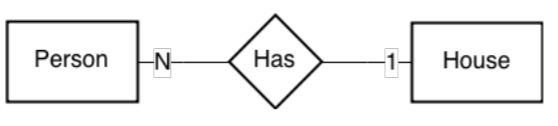
\includegraphics[scale=0.8]{src/L10I1.PNG}
\end{center}
Rectangles represent entities. Diamonds represent relationships. 1, N or M represent the cardinality of the relationship- N and M mean many. In the example above, we have a one-to-many relationship. A house has many people, but a person only has one house.

\noindent A many-to-many relationship is depicted below:
\begin{center}
    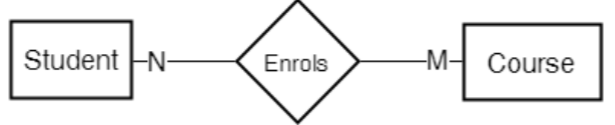
\includegraphics[scale=0.8]{src/L10I2.PNG}
\end{center}
Here, we say that a student can enrol into many courses, and a course can have many students enrolled in it.

\noindent Chen notation shows attributes as circles/ellipses, e.g.
\begin{center}
    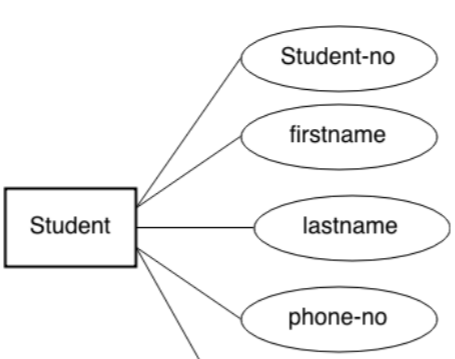
\includegraphics[scale=0.8]{src/L10I3.PNG}
\end{center}
This gets pretty cumbersome. On the other hand, in compressed Chen notation, we only put entities and relationships in the diagram. Then, we separately list the attributes, e.g.
\begin{center}
    \begin{tabular}{|c|c|}
        \hline
        Field & Type \\
        \hline
        Student No & Char (8) \\
        \hline
        FirstName & Char(128) \\
        \hline
        SecondName & Char(128) \\
        \hline
        Phone-no & Char(15), formatted \\
        \hline
    \end{tabular}
\end{center}
This way, we can neatly represent the attributes and their types.

\subsection{Relations in Django Models}
In Django, every \texttt{model} is automatically assigned an \texttt{id}. To create relationships between models, we refer to the \texttt{model}, not the \texttt{id}. For example, given the \texttt{House} model, the \texttt{Person} class becomes:
\begin{lstlisting}[language=python]
class Person(models.Model):
    house = models.ForeignKey(House)
\end{lstlisting}
By writing this code in the \texttt{Person} class, we know that it is the \texttt{Person} that is many (i.e. many people live in the same house). In Rango, the \texttt{Category} and \texttt{Page} models also share a relationship, as we can see below:
\begin{lstlisting}[language=python]
class Category(models.Model):
    name = models.CharField(max_length=128, unique=True)
    views = models.IntegerField(default=0)
    likes = models.IntegerField(default=0)
    slug = models.SlugField(blank=True, unique=True)

class Page(models.Model):
    category = models.ForeignKey(Category)
    title = models.CharField(max_length=128)
    url = models.URLField()
    views = models.IntegerField(default=0)
\end{lstlisting}
Here, a category can have many pages, but a page belongs to one category.

\noindent Now, assume we want to represent a one-to-one model with entities \texttt{Place} and \texttt{Restaurant}:
\begin{lstlisting}[language=python]
from django.db import models

class Place(models.Model):
    name = models.CharField(max_length=50)
    address = models.CharField(max_length=80)

class Restaurant(models.Model):
    place = models.OneToOneField(Place,
        on_delete=models.CASCADE, primary_key=True
    )
    serves_hot_dogs = models.BooleanField(default=False)
    serves_pizza = models.BooleanField(default=False) 
\end{lstlisting}
The reason we add a \texttt{place} field within \texttt{Restaurant} (and not the other way round) is that the \texttt{Place} need not be a \texttt{Restaurant}, but a \texttt{Restaurant} needs to be a \texttt{Place}. In Django, primary keys are normally auto-assigned integers, but here the primary key of a restaurant is its \texttt{Place}.

\noindent Next, we represent a many-to-one relationship with the entities \texttt{Reporter} and \texttt{Article}:
\begin{lstlisting}[language=python]
from django.db import models

class Reporter(models.Model):
    first_name = models.CharField(max_length=30)
    last_name = models.CharField(max_length=30)
    email = models.EmailField()
    
class Article(models.Model):
    reporter = models.ForeignKey(Reporter, 
        on_delete=models.CASCADE)
    headline = models.CharField(max_length=100)
    pub_date = models.DateField()
\end{lstlisting}
This model represents that a reporter can write many articles, but one article can only be written by a reporter.

\noindent Finally, we represent a many-to-many relationship with entities \texttt{Publication} and \texttt{Article}:
\begin{lstlisting}[language=python]
from django.db import models

class Publication(models.Model):
    title = models.CharField(max_length=30)

class Article(models.Model):
    publications = models.ManyToManyField(Publication)
    headline = models.CharField(max_length=100)
\end{lstlisting}
Instead of adding the \texttt{publications} field in the \texttt{Article} class, we could have also added the \texttt{articles} field in the \texttt{Publication} class.
\newpage

\section{Cascading Style Sheets}
Whilst developing web applications, the minimum useful set of technologies for a sufficiently complex application is five:
\begin{itemize}
    \item Server-side language (e.g. PHP, Ruby, Python, Java, etc.);
    \item Data Language (e.g. SQL);
    \item Client Language (e.g. JavaScript);
    \item Content Markup Language (e.g. XHTML); and
    \item Style Markup Language (e.g. CSS)
\end{itemize}
This turns out to be a headache when developing, especially when the languages mix together in one web page/file. Maintenance becomes particularly difficult and the codebase is especially fragile to change.

\noindent With the separation of concerns, our 3-tier diagram is:
\begin{center}
    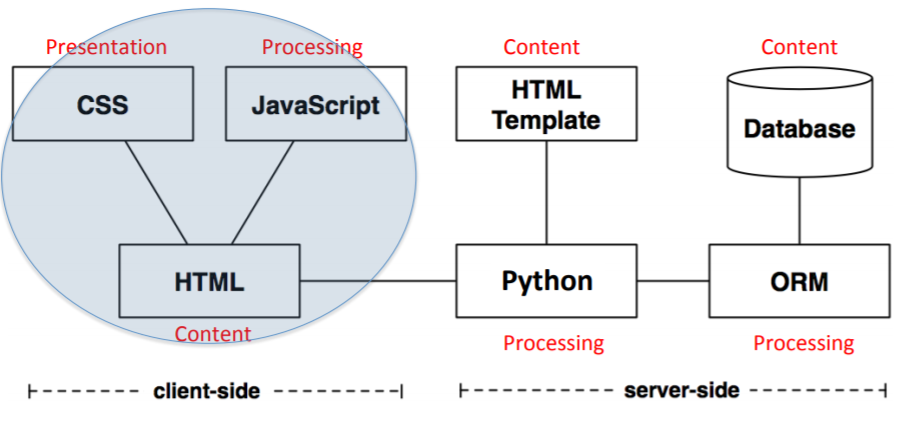
\includegraphics[scale=0.6]{src/L10I5.PNG}
\end{center}
We have separated the presentation, content and processing on the client side. 

\noindent We will focus on style on the web now. Most aspects about of any element of a web page can be controlled, e.g. position, colour, size, font, etc. This can be achieved in a lot of ways:
\begin{itemize}
    \item We can use Cascading Style Sheets (CSS) in combination with (X)HTML;
    \item We can describe the page in XML and then use XSL to generate formatted XHTML; or
    \item We can use Cascading Style Sheets (CSS) in combination with XML.
\end{itemize}
We are only going to look at the top way.

\noindent Stylesheets describe the rendering of html elements. They specify stylistic aspects of individual elements or all elements of a particular kind. CSS consists of a set of formatting rules, which are specified in the following way:
\begin{lstlisting}
selector {
    property1: value1;
    property2: value2;
    ...
}
\end{lstlisting}
The selector indicates the element (or set of elements). The property refers to the stylistic aspect, while the value is the specific configuration. An example of this is:
\begin{lstlisting}
h3 {
    color: yellow;
    size: 18px;
}
\end{lstlisting}
Here, the selector is the \texttt{h3} tag. We are setting the font colour to be yellow and font size to be 18 pixels. This now applies to every \texttt{h3} tag. It finds and applies patterns, as illustrated below:
\begin{lstlisting}[language=java]
/** Applies to all <p> elements **/
p {
    font-size: 12pt;
    font-face "Verdana";
}

/** Applies to all <h1>, <h2>, <h3> elements **/
h1, h2, h3 {
    color: red;
    font-size: 18px;
}

/** Applies to all elements **/
* {
    text-align: left;
}

/** Applies to all elements with id = "menu" **/
#menu {
    padding: 45px 25px 0px 25px;
    border: none;
    height: 80px;
}
\end{lstlisting}

\subsection{Values and Units}
Units affect the colours, distances and sizes of a whole host of properties of an element's style. 

\noindent We can specify numbers, which can be integers or real numbers. 

\noindent We can also use percentages, which is a real number followed by \%. It is generally relative to some other number, e.g. \texttt{font-size: 90\%} is relative to the default or the inherited style. 

\noindent We can also specify \texttt{color} by name (e.g. \texttt{red}). We can also specify it functionally (e.g. \texttt{rgb(255, 0, 0)}), or by hexadecimal RGB codes (\texttt{\#FF0000}).

\noindent Lengths can be given with normal units such as inches (in), centimeters (cm), milimeters (mm), points (pt, where 72pt = 1in), and picas (pc, where 1pc = 12pt).

\noindent We also have relative length units. For example, em is relative to the given font-size, i.e. if \texttt{font-size} is 14pt, then 1em = 14pt. The unit ex is relative to the size of a lowercase x for the given font-family. Also, the unit px is related to the size of a pixel on the device. It is generally the recommended unit to use.

\subsection{CSS and HTML}
There are 3 ways of using CSS in HTML documents:
\begin{itemize}
    \item Inline CSS Specification. Inline means that the style information is added directly to a particular element using the \texttt{style} attribute. CSS syntax is used with the attribute in an HTML tag, e.g.
    \begin{lstlisting}[language=html]
<h3 style="color: yellow; font-size: 18px;">\end{lstlisting}
    This only affects this element, and others of the same type are not affected. This approach is useful to override existing style, but it breaks the separation of content and presentation.
    
    \item Embedded CSS Specification. Embedded means that the style rules can be specified in the \texttt{head} section of the document. These rules will be applied to the entire document. An example of this is:
    \begin{lstlisting}[language=html]
<html>
<head>
    <style>
        h3 {
            color: yellow;
            font-size: 18px;
        }
    </style>
</head>
<body>
    <h3>This text will appear blue and 18px</h3>
</body>
</html>\end{lstlisting}
    It is still in the same document, so we might have a lot of duplicate code if there are many html files.
    
    \item External CSS Specification. External means that the CSS is in a separate document which can be shared by several pages. The extension of the file is `.css'. We import the file as follows:
    \begin{lstlisting}[language=html]
<head>
    <link rel="stylesheet" href="master.css" type="text/css">
</head>\end{lstlisting}
    This is generally the best method in terms of separation of concerns, ma-intenance and performance.
\end{itemize}

\subsection{Specialisation of Presentation}
\subsubsection{Class and ID Selectors}
Class and ID selectors can be used for finer control. This involves more planning and effort with document markup. But, it can result in a better user experience. It is also very important for manipulating elements in JavaScript. The effort also pays off if we use libraries such as jQuery.

\noindent Class selectors work on a set of specified elements through the class attribute. On the other hand, ids provide a way to stylise unique elements through the id attribute.

\noindent Class selectors allow us to style items with the same HTML element differently. They work when the class attribute of an HTML tag is given a name. The dot (\texttt{.}) operator is used to reference the class. The example below uses class selectors:
\begin{lstlisting}[language=html]
<style>
    .warning {
        font-weight:bold;
    }
</style>

<p class="warning">This text will be displayed in bold.</p>
<p> This text will not be displayed in bold.</p>
<p class="warning">Bold again here.</p>
\end{lstlisting}

\noindent ID selectors are similar to class selectors, but they define a special case for an element. IDs are meant to be unique and only used once. However, browsers are not particularly fussy about enforcing the uniqueness of identifiers (although it becomes difficult to recognise errors if we are use the same id more than once). The hash symbol (\texttt{\#}) is used to specify a unique ID. The example below uses id selectors:
\begin{lstlisting}[language=html]
<style>
    #first-para {
        font-weight: bold;
    }
</style>

<p id="first-para">This paragraph will be bold-faced.</p>
<p>This will not be bold.</p>
<p id="third-para">This will not be bold either</p>
\end{lstlisting}

\subsubsection{Descendent selectors}
Elements that are descended from a particular element are styled according to the rule of the descendent selector. This means that the rules will not be applied to a set of elements in one context, but not in another. For example, consider the following code:
\begin{lstlisting}[language=html]
<style>
    p em {
        color: red;
        font-weight: bold;
    }
</style>

<p>
    This will be the default colour.
    <em>This will be red, bold and italics.</em>
    Back to the default colour.
</p>
\end{lstlisting}
We can combine this with classes as well. Consider the following 3 subtleties:
\begin{itemize}
    \item Assume we have the following code in our HTML document:
    \begin{lstlisting}[language=html]
<style>
    .red h2 {
        color: red;
    }
</style>

<div class="red>
    <h2>I am red</h2>
</div>\end{lstlisting}
    Then, all \texttt{h2} elements within the class \texttt{red} will be coloured red.
    \item Next, assume we have the following code in our HTML document:
    \begin{lstlisting}[language=html]
<style>
    h2.red {
        color=red;
    }
</style>

<h2 class="red">I am red</h2>\end{lstlisting}
    Then, all \texttt{h2} elements whose class is red will be coloured red.
    \item Finally, assume we have the following code in our HTML document:
    \begin{lstlisting}[language=html]
<style>
    #red h2 {
        color: red;
    }
    
    <div id="red>
        <h2>I am red</h2>
    </div>
</style>
    \end{lstlisting}
    Then, all \texttt{h2} elements within an element with ID \texttt{red} will be coloured red.
\end{itemize}

\subsubsection{Inheritance of style}
The order of the application of styles is through inheritance. Styles are applied not only to a specific element, but also to its descendants. For example, consider the code below:
\begin{lstlisting}[language=html]
<style>
    p {
        color: red;
        font-weight: bold;
    }
</style>

<p>Happily red. <em>Really emphasising redness.</em></p>
\end{lstlisting}

\subsubsection{Specificity of Style}
Sometimes, multiple rules apply to the same element. CSS uses a weighting scheme to ensure that there are predictable outcomes with conflicts of style. It is made up of the following rules:
\begin{itemize}
    \item For every ID attribute given in a selector, add (1, 0, 0). 
    \item For every class attribute value, attribute selection, or pseudo-class given in the selection, add (0, 1, 0).
    \item For every element and pseudo-element given in the selector, add (0, 0, 1).
\end{itemize}
We use ordering, then lexicography to resolve conflicts, e.g. (1, 0, 0) beats (0, 5, 5). Some examples are given below:
\begin{lstlisting}[language=java]
/** specificity = (0, 0, 1) **/
h1 {
    color: red;
}

/** specificity = (0, 0, 2) **/
body h1 {
    color: green;
}

/** specificity = (1, 0, 1) **/
#content h2 {
    color: silver;
}

/** specificity = (0, 1, 1) **/
h2.grape {
    color: purple;
}
\end{lstlisting}
Inline CSS overrides all of these- it is effectively (1, 0, 0, 0).

\noindent Even with the system above, we can still run into conflicts between two or more rules when they all have the same weight. CSS is based on a method of causing styles to cascade together, which is made possible by inheritance, specificity and order. The purpose of ``cascading'' is to find one winning rule among a set of rules that apply to a given element.

\noindent The following are the cascading rules:
\begin{itemize}
    \item We find all rules that contain a selector that matches a given element.
    \item We sort all declarations by explicitly weight applying to the element. Tho-se rules marked by \texttt{important} are given a higher weight, e.g.
    \begin{lstlisting}[language=java]
p {
    color: gray !important;
}\end{lstlisting}
    \item We sort all declarations by specificity applying to a given element. Those elements with higher specificity have more weight than those with lower specificity.
    \item Finally, we sort all declarations by order applying to a given element. Th-e later a declaration appears in the style sheet or document, the more weight it is given. Declarations that appear in an imported style sheet are considered to come before all declarations within the style sheet that imports them. 
\end{itemize}

\subsection{Page Layout}
Layout of major elements on a webpage (e.g. columns, navigation bars, sidebars, headers and footers) can be specified using CSS. Nowadays, the preferred solution is to divide a page into a collection of \texttt{div} elements.

\noindent CSS floating properties allow us to float elements horizontally (left and right, not up and down). Elements after the floating element will float around. So, if the screen size changes, the elements will move down. For example,
\begin{lstlisting}[language=html]
<head>
    <style>
        .thumbnail {
            float: left;
            width: 110px;
            height: 90px;
            margin: 5px;
        }
    </style>
</head>
<body>
    <img class="thumbnail" src="clematis_small.jpg">
    <img class="thumbnail" src="clematis2_small.jpg">
    <img class="thumbnail" src="clematis3_small.jpg">
</body>
\end{lstlisting}
CSS positioning properties allow us to position an element. Elements can be positioned using: \texttt{top}, \texttt{bottom}, \texttt{left} and \texttt{right} properties. There are 4 different ways to position: \texttt{static} (default), \texttt{fixed}, \texttt{relative} and \texttt{absolute}. The CSS below illustrates this:
\begin{lstlisting}[language=java]
div {
    border: 1px solid #999999;
    margin: 20px;
}

div.fixed {
    position: fixed;
    top: 30px;
    right: 5px;
}

div.relative {
    position: relative;
    top: -50px;
}

div.absolute {
    position: absolute;
    left: 100px;
    top: 150px;
}
\end{lstlisting}
We now look at the 4 position values:
\begin{itemize}
    \item Static position is how HTML elements are positioned by default. A static-positioned element is always positioned according to the normal flow of the page. Static positioned elements are not affected by the \texttt{top}, \texttt{bottom}, \texttt{left} and \texttt{right} properties.
    \item An element with fixed position is positioned relative to the browser window. It doesn't matter if we scroll or resize. This might mean that it has to overlap with the other content.
    \item A relative-positioned element is positioned relative to its normal position.
    \item An absolution position element is positioned relative to the first parent element that has a position other than static.
\end{itemize}

\subsection{The Box Model}
Every element generates one or more rectangular element boxes which houses the content. The element box is surrounded by optimal amounts of padding, borders and margins, as shown below:
\begin{center}
    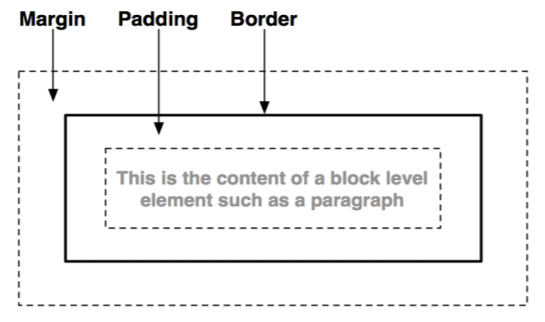
\includegraphics[scale=0.8]{src/L11I1.PNG}
\end{center}
The following labels the box model in more detail:
\begin{center}
    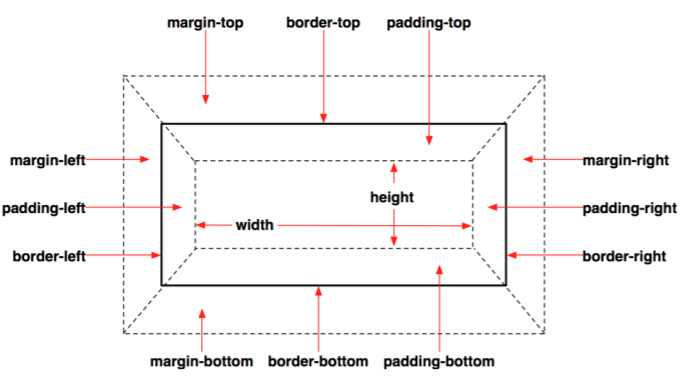
\includegraphics[scale=0.8]{src/L11I2.PNG}
\end{center}
Each of the labelled attribute above is a CSS property.

\noindent In summary, CSS is a method of separating a document's structure and content from its presentation. CSS allows for a much richer document appearance than HTML alone. CSS can save time as the appearance of the entire document can be created and changed in just one place. CSS can improve load times as it compactly stores the presentation concerns of a document in one place instead of being repeated throughout the document.

\noindent Separation of concerns is a good principle to adopt. We can see that the effort is worth it as the complexity increases. CS is a powerful method of specifying the style of web pages. It separates presentation from structure and concern.
\newpage

\section{JavaScript}
\subsection{Document Object Model}
The following is the 3-tier content:
\begin{center}
    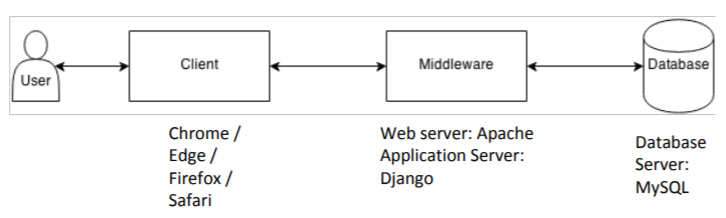
\includegraphics[scale=0.7]{src/L12I1.PNG}
\end{center}
In this chapter, we will look at the client. The clients can be a PC, Phone, Tablet or even embedded. We will focus on the document object model, which is a hierarchy of how the elements are arranged in a webpage.

\noindent The Document Object Model (DOM) is a platform- and language-neutral interface that will allow programs and scripts to dynamically access and update the content, structure and style of documents. The document can be further processed and the results of that processing can be incorporated back into the presented page.

\noindent In the HTML DOM, everything is a node. There are 5 types of nodes:
\begin{itemize}
    \item The document itself is a document node;
    \item All HTML elements are element nodes;
    \item All HTML attributes are attribute nodes;
    \item Text inside the HTML elements are text nodes;
    \item Comments are comment nodes.
\end{itemize}
Element nodes have child nodes. These are either element nodes, attribute nodes, text nodes or comment nodes. A NodeList object represents a list of nodes, like an HTML element's collection of child nodes.

\noindent The DOM has a hierarchical structure. For example, the following diagram pr-esents the code and the DOM for the code:
\begin{center}
    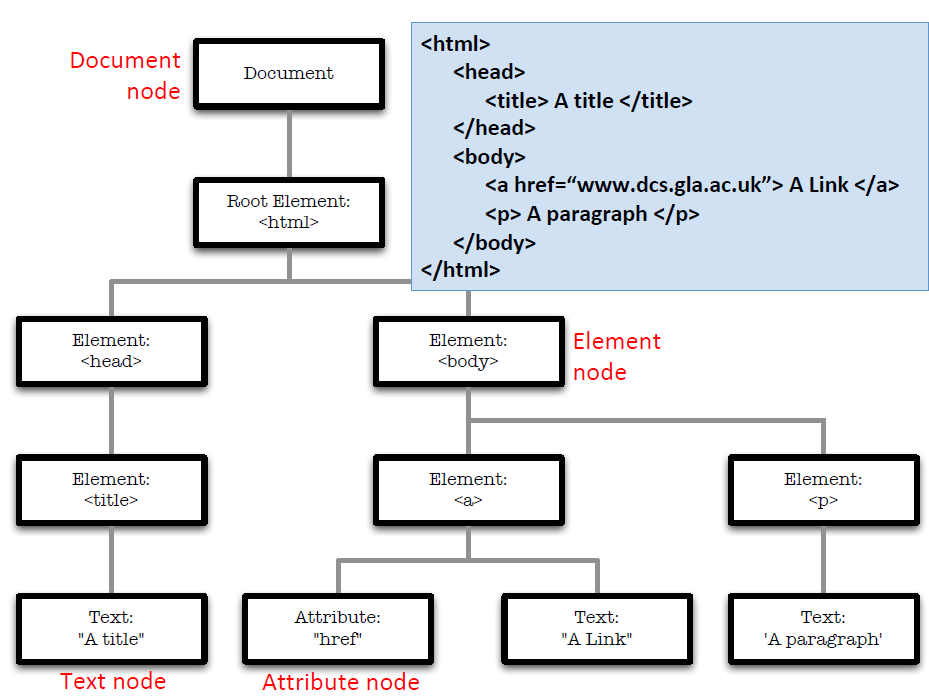
\includegraphics[scale=0.5]{src/L12I4.PNG}
\end{center}
We can traverse the DOM tree via pointers, as illustrated below:
\begin{center}
    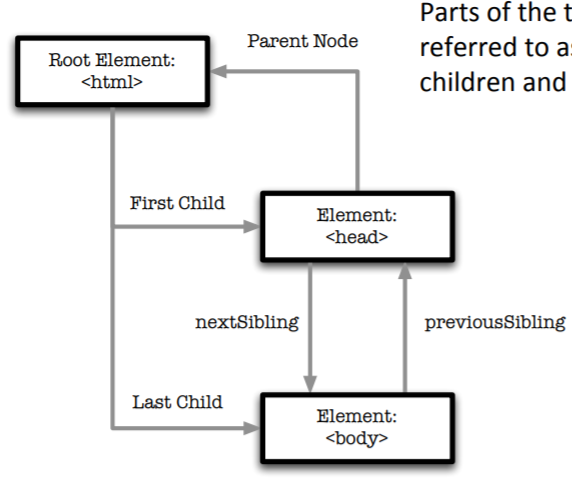
\includegraphics[scale=0.5]{src/L12I2.PNG}
\end{center}
Element within a DOM have the following properties:
\begin{itemize}
    \item The text value of the element, called its \texttt{innerHTML} property (within Java-Script);
    \item The name, called \texttt{nodeName};
    \item The value, called \texttt{nodeValue}. For elements, this is \texttt{null};
    \item The parent node, called \texttt{parentNode};
    \item The child nodes, called \texttt{childNodes}; and
    \item The attributes, called \texttt{attributes}.
\end{itemize}
Using JavaScript, we also have access to the following methods:
\begin{itemize}
    \item \texttt{getElementById}, which returns the element with a specified id;
    \item \texttt{getElementsByTagName}, which returns all the elements with a specified tag name;
    \item \texttt{appendChild}, which inserts the node provided; and
    \item \texttt{removeChild}, which removes the node provided.
\end{itemize}
There are many advantages to the DOM. The XML/tree structure makes the DOM easy to traverse- elements can be accessed one or more times. The structure of the tree is modifiable- values, elements and the structure can be added, changed or modified. It is a standard of the W3C, i.e. the unofficial-official law of the jungle.

\noindent There are also disadvantages to the DOM. It is resource-intensive and consumes a lot of memory- it needs to be fully loaded in main memory. It can be slow- the speed depends on the size and the complexity of the tree. It may not be the best choice for all devices and apps, i.e. a graphics intensive application or game may not be suited well to this model. A better alternative might be to use the Canvas directly, i.e. OpenGL.

\subsection{Event Handling}
When a user performs an action, an event is triggered. There are many ways for this to be triggered, e.g. \texttt{onKeyDown}, \texttt{onKeyUp}, \texttt{onClick}, \texttt{onSubmit}, \texttt{onFocus}, etc. These event objects are part of the DOM. The event object gives us the following information:
\begin{itemize}
    \item the target element in which the event occurred;
    \item the state of the keyboard keys;
    \item the location of the mouse cursor; and
    \item the state of the mouse buttons.
\end{itemize}
We can catch the event, e.g. user input from forms can be validated on the client-side using JavaScript:
\begin{lstlisting}[language=html]
<form name="login_form" onsubmit="validateForm()" method="post">
    Username: <input type="text" name="username">
    Password: <input type="password" name="password">
    <input type="submit" value="Submit">
</form>
\end{lstlisting}
The \texttt{onsubmit} attribute above takes in a boolean value, returning \texttt{true} if the form is valid. The function \texttt{validateForm()} must therefore validate the form and return \texttt{true} or \texttt{false} accordingly.

\noindent Each even object has an `event target', i.e. the node in the DOM tree from where an event originated. There are two main types of event flow- event capturing (global handling), or event bubbling (local handling). Eventflow follows a ``Rou-ndTrip'' pattern/model. This can be visualised as follows:
\begin{center}
    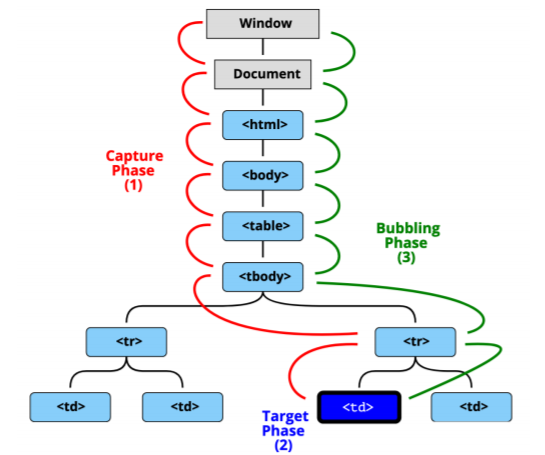
\includegraphics[scale=0.8]{src/L12I3.PNG}
\end{center}
In the image above, an event has occurred on the \texttt{td} element. The capture phase starts from the \texttt{Window} and we descend to the \texttt{td} element from there as we try to capture the event. In the bubbling phase, we start from the \texttt{td} element, and we would go up to the \texttt{Window}. We could have listened to this event in any of the DOMs within the traversal (e.g. the event would have been captured through the same event listener on the \texttt{tr} element as well).

\noindent Formally, the event propagates downwards through an element's ancestors. Any event listeners of the ancestor elements will be executed first. This is the event capture. During the event bubbling, the event propagates upwards through an element's ancestors. Any event listeners of the element will be executed first. Ancestors can then potentially handle the event.

\noindent To see this in action, consider the following HTML code:
\begin{lstlisting}[language=html]
<div onclick="function1()">
    <span onclick="function2()">
        <button onlick="function3()">Click here</button>
    </span>
</div>
\end{lstlisting}
Now, if the button gets clicked, we have two possibilities:
\begin{itemize}
    \item if the event is handled under event capture, \texttt{function1} runs first, then \texttt{function2} and finally \texttt{function3};
    \item if the event is handled under event bubbling, \texttt{function3} runs first, then \texttt{function2} and finally \texttt{function1}.
\end{itemize}
Both types of events are generated, but bubbling is caught by handles by default and is used more often in practice.

\noindent Now, assume we have the following HTML:
\begin{lstlisting}[language=html]
<html>
<head>
    <link rel="stylesheet" type="text/css" href="events.css">
</head>
<body>
    <div>1
        <div>2
            <div>3
                <div>4
                    <div>5</div> 
                </div>
            </div>
        </div>
    </div>
    <p id="log"></p>
    <script type="text/javascript" src="events.js"></script>
</body>
</html>
\end{lstlisting}
Now, assume the JavaScript file \texttt{events.js} has the following code:
\begin{lstlisting}[language=javascript]
var node = document.getElementById("log");
var divs = document.getElementsByTagName("div");

function append(line) {
    var text = node.innerHTML;
    node.innerHTML = text + "<p>" + line + "</p>";
}

function capture() {
    append("capture:" + this.firstChild.nodeValue);
}

function bubble() {
    append("bubble:" + this.firstChild.nodeValue);
}

for (var i = 0; i < divs.length; i++) {
    // "click" is the event type, capture/bubble are the functions 
    // from above, bool is useCaptureModel (defaults to false)
    divs[i].addEventListener("click", capture, true);
    divs[i].addEventListener("click", bubble, false);
}
\end{lstlisting}

\subsection{JavaScript}
The following is the high-level overview of client-side scripting:
\begin{center}
    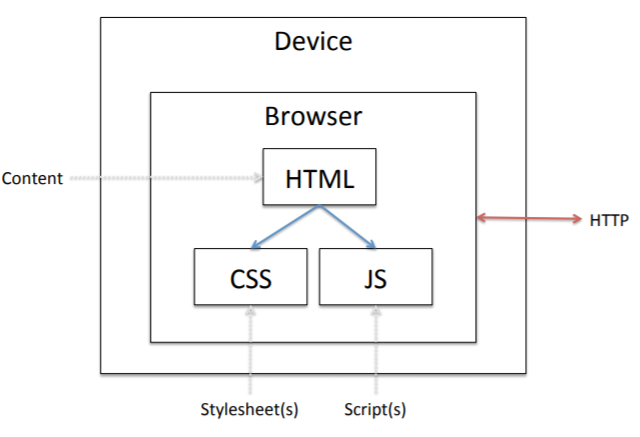
\includegraphics[scale=0.7]{src/L13I1.PNG}
\end{center}
The client is on some device, using some browser. The web app is composed of HTML (code), CSS (styling) and JS (functionality). 

\noindent We are going to focus on JavaScript now. It is a web-only programming language, though it is useful for a wide range of programming tasks (e.g. node.js). It looks like a procedural language, but it is closer to a functional language. Here, functions are first class citizens (functions can be arguments of other functions). It also supports anonymous functions, which is heavily used by jQuery. There is a standard form of JavaScript (ECMA).

\noindent There are some design errors in JavaScript. Small things annoy, such as semi-colon insertion and overloaded operators. Some problems can be avoided by using IDEs to check syntax, or JSLint.

\noindent JavaScript is syntatically similar to Java and C. There are familiar primitive data-types (e.g. numbers, strings and booleans). The language is object-oriented in its own way. It is an interpreted language (so no compiling). It has dynamic typing, and functions are first class citizens (we can have nested and anonymous functions as well).

\noindent Like CSS, JavaScript can also be added into an HTML document in 3 ways:
\begin{itemize}
    \item Inline JavaScript-scripts can be included inline with the HTML code, like in the following case:
    \begin{lstlisting}[language=html]
<html>
<head></head>
<body>
    <script type="text/javascript">
        document.writeln("Hello world!");
    </script>
</body>
</html>\end{lstlisting}
    This might be good for experimentations, but it violates separation of concerns and should be avoided.
    
    \item Embedded javascript- scripts can be added in HTML head, like in the following case:
    \begin{lstlisting}[language=html]
<head>
    <script type="text/javascript">
        function get_false() {
            return false;
        }
    </script>
</head>\end{lstlisting}
    It is fragile to maintain, like in the case of embedded CSS.
    
    \item External JavaScript- scripts can be kept in external files and linked to the \texttt{headd} section, like in the following case:
    \begin{lstlisting}[language=html]
<html>
<head>
    <script type="text/javascript" src="script.js"></script>
</head>
<body></body>
</html>\end{lstlisting}
    This is easier to manage over time.
\end{itemize}

\subsection{DOM Integration}
The intent behind JavaScript was to dynamically script and manipulate documents. HTML documents are modelled using the DOM. DOM methods and properties can be accessed and altered using JavaScript. For example, let's consider the following JavaScript code:
\begin{lstlisting}[language=javascript]
// Find the number of tables in a document
var tables = document.getElementsByTagName("table");
alert("This document contains " + tables.length + " table(s)");

// Find a specific table within a document and count its rows
var tableOfContents = document.getElementByID("TOC");
var rows = tableOfContents.getElementByTagName("tr");
var numrows = rows.length;
\end{lstlisting}

\noindent The real impact of JavaScript is changing the content of the DOM, as shown below:
\begin{lstlisting}[language=javascript]
// This function traverses the DOM tree and
// converts all text node data to uppercase
function upcase(n) {
    if (n.nodeType == 3 /** Node.TEXT_NODE **/) {
        n.nodeValue = n.nodeValue.toUpperCase();
    } else {
        var children = n.childNodes;
        for (var i = 0; i < children.length; i++) {
            upcase(children[i]);
        }
    }
}
\end{lstlisting}
The method \texttt{Node.nodeType} returns an integer, which corresponds to the following nodes:
\begin{itemize}
    \item 1 refers to an element node;
    \item 2 refers to an attribute node;
    \item 3 refers to a text node;
    \item 8 refers to a comment node; and
    \item 9 refers to a document node.
\end{itemize}

\noindent If we want to run the function \texttt{upcase} and make all the text within a webpage upper case, then we need to call the function \texttt{upcase} at the bottom of the document body. The only nodes that are affected by the function are those above the line where we call the function.

\subsection{JavaScript Syntax}
JavaScript is a case-sensitive language (keywords, identifiers, variables, functions, etc. must be consistent). Whitespace is ignored (spaces, tabs and newlines). However, semicolons are options, but good practice. JavaScript interpreters automatically add them- this is a very bad thing, so it is better to be explicit. So, assume we have the following JavaScript code:
\begin{lstlisting}[language=javascript]
return
true;
\end{lstlisting}
Then, JavaScript interpreters register the code as:
\begin{lstlisting}[language=javascript]
return;
true;
\end{lstlisting}
Therefore, \texttt{undefined} gets returned- not \texttt{true}.

\noindent Comments can be single \texttt{//}, or multiline \texttt{/* */}. Literals are data values that appear directly in the language: \texttt{12}, \texttt{1.2}, \texttt{''hello''}, \texttt{true}, etc. Identifiers are names for variables and functions. The first character must be letter, underscore or dollar. Remaining characters can include above and numbers. We cannot use reserved words as identifiers. 

\subsubsection{Primitive and Trivial Types}
There are 3 primitive types in JavaScript:
\begin{itemize}
    \item Number- there is no distinction between integers, decimal and floating point values;
    \item String- sequence of unicode letters, digits and punctuation characters delimited by single or double quotes;
    \item Boolean- \texttt{true} or \texttt{false}.
\end{itemize}
We also have two trivial types:
\begin{itemize}
    \item The value \texttt{null} represents no value- it is (a placeholder) for an object;
    \item The value \texttt{undefined} represents a variable that has been declared but not assigned a value. It can also be used for an object property that does not exist.
\end{itemize}

\subsubsection{Functions}
A JavaScript function is a piece of executable code that is defined once, but can be called multiple times. In other languages, functions (or methods) are often just useful construct to gather related code. However, in JavaScript, functions are first class objects in the language, and can be passed as datatypes. The following has two examples of function usage in JavaScript:
\begin{lstlisting}[language=javascript]
var square = function (x) {
    return x * x;
}

// y = 16
y = square(4);

function sq(x) {
    return x * x;
}

function applyOperator(op, x) {
    return op(x);
}

// y = 16
y = applyOperator(sq, 4);
\end{lstlisting}

\subsubsection{Objects}
An object is a collection of named values. Named values are known as the object's properties. Objects are created by invoking a constructor or using the object literal short-hand syntax.
\begin{lstlisting}[language=javascript]
function point(xVal, yVal) {
    this.x = xVal;
    this.y = yVal;
}

var p1 = new point(2.5, 5.4);

var p2 = new Object();
p2.x = 2.5;
p2.y = 5.4;

var p3 = {x: 2.5, y: 5.4};
\end{lstlisting}
The objects \texttt{p1}, \texttt{p2} and \texttt{p3} are the same.

\subsubsection{Arrays}
Arrays are also very similar to Objects, acting as a collection of data values. For objects, each value has a name (\texttt{obj.x}), while arrays have an index (\texttt{arr[0]}) instead. The elements in the array do not have to have the same type, and their size is dynamic. There are many methods defined on arrays, such as join, reverse, sort, concat, splice, push and pop.
\begin{lstlisting}[language=javascript]
var a1 = new Array();
a1[0] = 120;
a1[1] = "hello";

a2 = [120, "hello"];
\end{lstlisting}
The arrays \texttt{a1} and \texttt{a2} are the same.

\subsubsection{Variables}
Variables are identifiers associated with a value. It is used to store and manipulate values in a program. All variables are untyped (weak or loose typing). Variables are declared using the \texttt{var} keyword. If this is missing, then the variable is global (this is not recommended). The scope of the variables depends on where they are declared:
\begin{itemize}
    \item Global variables can be seen everywhere;
    \item Variables declared in a function are only visible locally;
    \item Omitting \texttt{var} in functions will use matching global variables; and
    \item There is no block sope like C/Java languages.
\end{itemize}
For example, consider the following code:
\begin{lstlisting}[language=javascript]
var i = 10;
var j = 10;

function scope() {
    i = "Hello";
    var j = "Hello";
}

scope();
// i is "Hello"
// j is 10
\end{lstlisting}

\subsubsection{Expressions}
An expression is a phrase of code that can be evaluated to produce a value, as shown below:
\begin{lstlisting}[language=javascript]
1.5                             // a numeric literal
"hello"                         // a string literal
True                            // a boolean literal 
/java/                          // a regexp literal
{x: 1, y: 2}                    // an object literal
[1, 2, 3, 4, 5]                 // an array literal
function (x) {return x*x;}      // a function literal
sum                             // the variable sum
\end{lstlisting}
Simple expressions can be combined using operators. JavaScript supports a common set of operators, e.g. arithmetic (\texttt{+}), equality (\texttt{==}, \texttt{===}), relational (\texttt{>}) and logical (\texttt{\&\&}). We must take care when using operators. For example, \texttt{+} can mean addition of numbers, but also concatenation of strings. Also, \texttt{==} tests for equality, while \texttt{===} tests for both equality and type.

\subsubsection{Statements}
The following are statements in JavaScript:
\begin{lstlisting}[language=javascript]
// expression statement
var x = 1 + 2;

// if/else-if/else statement
if (condition) {
    statement;
} else if (condition) {
    statement;
} else {
    statement;
}

// while statement
while (condition) {
    statement;
}

// for statement
for (var i = 0; i < 10; i++) {
    statement;
}

// function statement
function name(args) {
    statement;
}

// try-catch-finally statement
try {
    // Normally, this code runs from top to bottom.
    // Sometimes, an exception may be thrown
    // either directly with a throw statement,
    // or indirectly by calling another method.
} catch (e) {
    // The statements here are executed if and only if
    // the try statement generated an exception.
    // These statements handle the exception somehow.
} finally {
    // The statements here are always executed
    // regardless of what happened in the try-block
}
\end{lstlisting}

Objects are unordered collections of properties. Beside using the `dot' operator to access properties, we can also use the \texttt{[...]} operator. As JavaScript is dynamic and objects can have properties added at any time, this is a very convenient method, for example:
\begin{lstlisting}[language=javascript]
var cust = new Object();
cust.addr0 = "36 King St";
cust.addr1 = "42 Queen Rd";
cust.addr2 = "16 Abbey St";

var addr = "";
for (var i = 0; i < 3; i++) {
    addr += cust["addr" + i] + "\n";
}
\end{lstlisting}
Functions in JavaScript can also be nested. They support optional arguments- if it is invoked with fewer arguments, the remaining arguments are \texttt{undefined}. The arguments object can be used with variable length argument lists, e.g. the function object has a property arguments which can be inspected to find which and how many arguments were given. Functions that are properties of objects are usually referred to as methods.

\subsubsection{Classes}
The following code defines a class in JavaScript:
\begin{lstlisting}[language=javascript]
class Rectangle {
    constructor (idString, widthVal, heightVal) {
        this.id = idString;
        this.resize(widthVal, heightVal);
    }
    
    resize(widthVal, heightVal) {
        this.width = widthVal;
        this.height = heightVal;
    }
    
    getArea() {
        return this.width * this.height;
    }
}

var rect = new Rectangle("Test", 4, 5);
document.writeln(rect.id);
document.writeln(rect.getArea());
rect.resize(6, 7);
document.writeln(rect.getArea());
\end{lstlisting}

\subsubsection{Regexp}
A regular expression (regexp) is an object that describes a pattern of characters that can be used to perform pattern matching and search and replace actions on text. Often, regexps can be though of as programs within a program. However, despite their utility, they can be a documentation nightmare.

\noindent In JavaScript, regexp are represented by \texttt{RegExp} objects. The following describes the syntax of regexp:
\begin{lstlisting}[language=javascript]
// syntax of a regexp => /pattern/modifiers
var re1 = /Free/i;
// "Free" pattern, "i" modifier (case insensitive)
var re2 = /s$/;
// match any string that ends with "s"
\end{lstlisting}
Next, we look at methods that we can call using \texttt{RegExp}:
\begin{itemize}
    \item \texttt{String.search(RegExp)}, which returns the starting position of the first match, or -1. For example,
    \begin{lstlisting}[language=javascript]
var str = "Visit W3Schools";
var n = str.search(/w3schools/i);
// n == 6\end{lstlisting}
    
    \item \texttt{RegExp.exec(String)}, which returns the first match, or \texttt{null}:
    \begin{lstlisting}[language=javascript]
var str = "Visit W3Schools";
var match = /w3schools/i.exec(str);
// match == "W3Schools"\end{lstlisting}

    \item \texttt{RegExp.test(String)}, which returns \texttt{true} if there is a match, and \texttt{false} otherwise:
    \begin{lstlisting}[language=javascript]
var str = "Visit W3Schools";
var match = /w3schools/i.test(str);
// match == true\end{lstlisting}
\end{itemize}
\newpage

\section{JQuery}
Despite JavaScript and DOM being functionally useful, coding on the client-side is not particularly easy. DOM scripting entails a lot of repetitive domain-specific boilerplate coding. A solution to this is a standard library. This would focus on the domain-specific programming tasks. One of these solutions is jQuery.

\noindent JQuery is one of the most popular JS libraries. It simplifies client-side scripting by:
\begin{itemize}
    \item selecting DOM elements;
    \item creating UI animations and effects;
    \item handling events;
    \item developing AJAX applications.
\end{itemize}
JQuery takes a lot of the problems out of developing for multiple browsers. It acts as a layer of abstraction over various browsers. There is no more browser sniffing. JQuery creates a useful foundation for additional functionality to be added. A wide range of specialised plug-ins have been developed since the release of jQuery for all manner of web-dev tasks (e.g. jQueryUI).

\noindent JQuery uses a basic pattern of selecting and adding on a particular DOM element and manipulating its parameters. We look at many jQuery examples below:
\begin{lstlisting}[language=javascript]
// change the text of an element with id = name to "the new text"
$("#name").text("the new text");

// set the color style of all the p elements blue
$("p").css("color", "blue");

// when the page loads, show the alert message
$(document).ready(function() {
    alert("Hello World!");
});

// do this after the page loads: when a link gets clicked, 
// show the alert message
$(function() {
    $("a").click(function() {
        alert("Hello World!");
    });
});

// do this after the page loads: when the button with id 
// toggleButton gets clicked, change the style of the p tag 
// with id text to font size 36 and text colour blue
$(document).ready(function() {
    $("#toggleButton").click(function() {
        $("p#text").css({
            fontSize: 36,
            color: "blue"
        });
    });
});

// when the element with id toggle button is clicked, set the 
// onclick event listener to the p element with id disclaimer which
// hides/shows it depending on whether it is visible right now
$("#toggleButton").click(function() {
    $("p#disclaimer").click(function() {
        if ($("#disclaimer").is(":visible")) {
            $("#disclaimer").hide();
        } else {
            $("#disclaimer").show();
        }
    });
});

// when an element with class bigtext is hovered, we move it by 30 
// pixels to the right; if it stops being hovered, we move it back
$(".bigtext").hover(function() {
    $(this).animate({
        paddingLeft: '+=30px'
    }, 200);
}, function() {
    $(this).animate({
        paddingLeft: '-=30px'
    }, 200);
});

// change the background colour of all the p tags depending on the event
$("p").on({
    mousenter: function() {
        $(this).css("background-color", "red");
    },
    mouseleave: function() {
        $(this).css("background-color", "green");
    },
    click: function() {
        $(this).css("background-color", "yellow");
    }
})

// when the form element with id myForm gets submitted,
// validate it
$("form#myForm").submit(function() {
    ("form#myForm").validate();
});

// after the page loads, whenever a button gets clicked, we move
// all the divs to right (slowly), make the font bigger, increase 
// the height, and then restore the original position
$(document).ready(function(){	
	$("button").click(function(){	
		var	div	= $("div");			
		div.animate({left: '100px'}, "slow");	
		div.animate({fontSize: '3em'}, "slow");	
		div.animate({height: '200px'}, "slow");	
		div.animate({left: '8px'}, "slow");	
		div.animate({fontSize: '1em'}, "slow");	
        div.animate({height: '100px'}, "slow");
    });	
});

// when the button with id btn1 gets clicked, we add a bold element
// to the end of all the p elements
$("button#btn1").click(function() {
    $("p").append("<b>Appended Text</b>");
});

// when the button with id btn2 gets clicked, we add a bold item
// to the end of all the ol elements
$("button#btn2").click(function() {
    $("ol").append("<li><b>Appended item</b></li>");
});
\end{lstlisting}
\newpage

\section{XML and JSON}
\subsection{XML}
XML stands for eXtensible Markup Language. It was designed to transport and store data. The design goals of XML emphasise simplicity, generality and usability.

\noindent XML was created because markup on the web was not being properly supported. Standard generalized markup language (SGML) was too complex, while HTML was too limited and mixed format with structure. XML aimed to:
\begin{itemize}
    \item provide a simpler markup language;
    \item separate language from structure;
    \item be extensible and provide support for a host of applications; and
    \item transport and store data.
\end{itemize}
We use it to describe the structure of semi-structured documents. It is a mechanism for sharing, transporting and storing annotated data. It aims to be a general purpose language for data description and interchange. XML has emerged as a dominant standard. It has additional tools for additional layers of processing, such as the ability to add formatting to XML documents, querying XML documents, transforming XML documents, and so on. XML can be extended to describe the data within specific domains, e.g. XHTML (for web pages), Wireless Markup Language (WML), MathML, etc.

\noindent The following is a sample XML file:
\begin{lstlisting}[language=xml]
<?xml version="1.0" encoding "UTF-8"?>
<breakfast_menu>
    <food>
        <name>Belgian Waffles</name>
        <price>$5.95</price>
        <calories>650</calories>
    </food>
    <food>
        <name>Strawberry Belgian Waffles</name>
        <price>$7.95</price>
        <calories>900</calories>
    </food>
</breakfast_menu>
\end{lstlisting}
Line 1 is called the prologue. The main body starts at line 2. The root here is \texttt{breakfast\_menu}. It looks very similar to HTML- nested tags, but based on a breakfast menu instead of a webpage here.

\noindent HTML was designed to display data. So, HTML elements mix format and structure with content and presentation. However, in XML, tags define the structure, and any presentation is handled separately. Therefore, the structure of XML is tightly controlled. Tags are case sensitive and variable values must be quoted. If there is a start tag, there must be an end tag. A hierarchical structure of elements is enforced. These are not strictly enforced in the case of HTML. XML does however provide flexibility- new tags (and variables) can be created by the programmer.

\noindent An XML document is made up of 3 parts:
\begin{itemize}
    \item An optional prolog- the XML declaration. It is composed of the version (must be 1.0 or 1.1), the encoding (how the characters are encoded in the file), and whether they are standalone (the value is yes if this document is entirely self-contained, and no if it has an external DTD or schema).
    \item The body- this contains the document elements and the data.
    \item An optional epilog- it contains comments and processing instructions.
\end{itemize}
The basic building blocks for XML are XML elements. An XML element is everything from (and including) the element's start tag to the element's final tag. An element can contain text, attributes, other elements, or a mixture of these. Element names are case sensitive. Closed elements consist of both opening and closing tags. Elements can be nested. All elements must be nested within a single root element. Nested elements are child elements. Empty elements are denoted by \texttt{<element></element>}, or just \texttt{<element/>}.

\noindent Attributes are characteristics of elements. They are case sensitive. The values of attributes must be in quotes, i.e. all values are text strings. Value can contain most characters and whitespace (but not the angle brackets and so on).

\noindent An XML document is well-formed if it satisfies the following:
\begin{itemize}
    \item XML tags are case-sensitive;
    \item For every start tag, there is an end tag;
    \item An XML parser will be able to process it and make use of the tree structure;
    \item XML attribute values must be quoted; and
    \item XML documents have to have a root element.
\end{itemize}

\subsubsection{DTD and Schema}
To share XML, a pre-defined structure can be used. These describe the tags which can appear, and can be done using Document Type Definitions (DTD), or XML schemas and XML namespaces. The XML can be checked according to the definitions and validated. These structures are references either at the top of the file or provided separately. An XML document is valid if it is well-formed and also conforms to the rules in the DTD or Schema.

\noindent The following is how we include DTD into an XML document:
\begin{lstlisting}[language=xml]
<?xml version="1.0"?>
<!DOCTYPE note [
<!ELEMENT note(to, from, heading, body)>
<!ELEMENT to(#PCDATA)
<!ELEMENT from(#PCDATA)
<!ELEMENT heading(#PCDATA)
<!ELEMENT body(#PCDATA)
]>
<note>
    <to>Bob</to>
    <from>Alice</from>
    <heading>Reminder</heading>
    <body>Cook dinner tonight!</body>
</note>
\end{lstlisting}
The root of the document is labelled by \texttt{DOCTYPE note}- it is \texttt{note} in this case. We specify that a note element must contain the elements \texttt{to}, \texttt{from}, \texttt{heading} and \texttt{body}. \texttt{\#PCDATA} means `parseable character data'.

\noindent The above was embedded DTD. We can put the DTD into another file, and reference it in the xml. For example, we can have the file \texttt{note.dtd} with the following:
\begin{lstlisting}[language=xml]
<?xml version="1.0"?>
<!ELEMENT note(to, from, heading, body)>
<!ELEMENT to(#PCDATA)
<!ELEMENT from(#PCDATA)
<!ELEMENT heading(#PCDATA)
<!ELEMENT body(#PCDATA)
\end{lstlisting}
Then, the \texttt{note.xml} file is:
\begin{lstlisting}[language=xml]
<?xml version="1.0"?>
<!DOCTYPE note SYSTEM "note.dtd">
<note>
    <to>Bob</to>
    <from>Alice</from>
    <heading>Reminder</heading>
    <body>Cook dinner tonight!</body>
</note>
\end{lstlisting}
We could have also used a schema here. For example, we can have the file \texttt{note.xsd} with the following schema:
\begin{lstlisting}[language=xml]
<xs:element name="note">
<xs:complexType>
    <xs:sequence>
        <xs:element name="to" type="xs:string"/>
        <xs:element name="from" type="xs:string"/>
        <xs:element name="heading" type="xs:string"/>
        <xs:element name="body" type="xs:string"/>
    </xs:sequence>
</xs:complexType>
</xs:element>
\end{lstlisting}
We can then reference the schema in the XML appropriately.

\noindent XML schemas are more powerful than DTDs. XML schemas are written in XML. XML schemas are extensible to additions. XML schemas support data types and namespaces. With XML schema, our XML files can carry a description of its own formation. Also, independent groups of people can agree on a standard for interchanging data. We can also easily verify data.

\subsubsection{XSL}
Extensible Stylesheet Language (XSL) is a styling language for XML. XSLT standards for XSL transformations. XSLT can be used to transform XML documents into other formats (e.g. XML to XHTML). 

\subsubsection{XHTML}
XHTML strict descends from XML, so we need to follow the XML rules within the HTML document. It separates visual rendering from the content- we cannot have style tags. There is a strict set of rules enforced on markup, e.g. the hierarchy is strictly enforced; all the tags must be lower case; and the placement of elements is restricted. An XHTML strict document will work in many different environments, e.g. visual browsers, braille readers, text-based browsers, print. It is highly configurable by the user and highly maintainable by the developer.

\noindent XML was designed to transport and store data, while HTML was designed to display data.

\subsection{JSON}
JavaScipt Object Notation (JSON) is an alternative to XML. It is a lightweight data interchange format. It is easy for humans to read and write. It is also easy for machines to parse and generate. There is less biolerplate, but there is more information per byte. JSON is built on two universal data structures- a collection of name/value pairs, or an ordered list of values. JSON is language independent.

\noindent The following is an example of a JSON file:
\begin{lstlisting}[language=javascript]
{
    "employees": [
        {
            "firstName": "John",
            "lastName": "Doe"
        },
        {
            "firstName": "Anna",
            "lastName": "Smith"
        },
        {
            "firstName": "Peter",
            "lastName": "Jones"
        }
    ]
}
\end{lstlisting}
In XML, this would be:
\begin{lstlisting}[language=xml]
<employees>
    <employee>
        <firstName>John</firstName>
        <lastName>Doe</lastName>
    </employee>
    <employee>
        <firstName>Anna</firstName>
        <lastName>Smith</lastName>
    </employee>
    <employee>
        <firstName>Peter</firstName>
        <lastName>Jones</lastName>
    </employee>
</employees>
\end{lstlisting}
JSON uses JavaScript syntax, but the JSON format is text only, just like XML. Text can be read and used as a data format by any programming language. JSON evaluates to JavaScript objects. The JSON format is syntactically identical to the code for creating JavaScript objects. Instead of using a parser (like XML does), a JavaScript program can use standard functions to convert JSON data into native objects.

\noindent The JSON syntax is derived from JavaScript object notation syntax:
\begin{itemize}
    \item Data is in name-value pairs, in the form \texttt{"name": "value"};
    \item Data is separated by commas;
    \item Curly brackets hold objects;
    \item Square brackets hold arrays.
\end{itemize}
JSON and XML are similar in many ways. They both are self-describing, and therefore human-readable. They are hierarchical, and can be parsed and used by a lot of programming languages. Both XML and JSON can be fetched with an \texttt{XMLHttpRequest}.

\noindent However, JSON and XML are also somewhat different. JSON doesn't use end tags. JSON is shorter, and therefore quicker to read and write. Also, JSON can use arrays.
\newpage

\section{AJAX}
Asynchronous JavaScript And XML (AJAX) is a key technology set underlying web apps. AJAX eliminates the need to reload a web server in order to get a new content from the server. This removes the start-stop interaction where a user has to wait for new pages to load. An intermediate layer (AJAX engine) is introduced into the communication chain between the client and the server. It improves the interactive experience in web apps.

\noindent AJAX provides the following technology set:
\begin{itemize}
    \item Standards-based presentation using (X)HTML and CSS;
    \item Dyanmic display and interaction using the DOM;
    \item Data interchange and manipulation using XML and XSLT;
    \item Asynchronous data retreival using \texttt{XMLHttpRequest}; and
    \item JavaScript binding everything together.
\end{itemize}
It can be written in `pure' JavaScript, jQuery or newer fetch API.

\noindent Previously, the client-server interaction could be described through the following image:
\begin{center}
    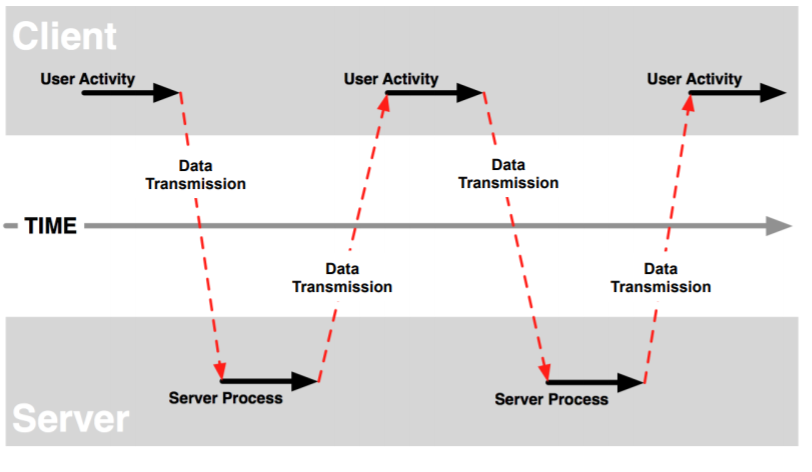
\includegraphics[scale=0.5]{src/L16I1.PNG}
\end{center}
This is the traditional client-server synchronous communication model. When a user performs an activity, data gets transmitted to the server. Then, the server returns some other data and completely replaces the webpage replacement. The cycle continuous and synchronous- only one of the client and server is working at one time.

\noindent We know that JavaScript can manipulate the DOM of a webpage to create, modify and remove content and style. The event handlers can be attached to events generated by the user and the browser. XML can model data and we can access it using the DOM. AJAX can also transport JSON or plain text.

\noindent The keystone of AJAX is \texttt{XmlHttpRequest} (XHT) object. The XHR is an object that is part of the DOM and is built into most modern browsers. It can communicate with the server by sending HTTP requests (much like normal client/server communication). It is independent of \texttt{form} or \texttt{a} elements for generating HTTP get and post requests. It does not block script execution after sending an HTTP request. As with content and style, JavaScript can now programmatically manage HTTP communication.

\noindent The updated communication model with AJAX is:
\begin{center}
    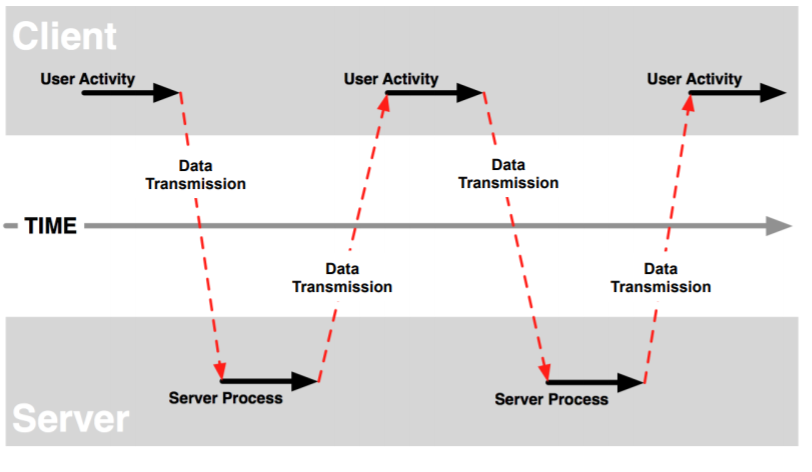
\includegraphics[scale=0.5]{src/L16I1.PNG}
\end{center}
So, the user request is being intercepted by the AJAX layer. It then decides when to communicate with the server, and what to do with the response.

\noindent We now consider how AJAX works in more detail:
\begin{itemize}
    \item An event occurs in a webpage (e.g. the page is loaded, a button is clicked);
    \item An \texttt{XMLHttpRequest} object is created by JavaScript;
    \item The \texttt{XMLHttpRequest} object sends a request to a web server;
    \item The server processes the request;
    \item The server sends a response back to the web page;
    \item The response is ready by JavaScript;
    \item Proper action (like page update) is performed by JavaScript.
\end{itemize}
We now look at the object \texttt{XmlHttpRequest}. It has the following properties:
\begin{itemize}
    \item The property \texttt{readyState} holds the status of the XMLHttpRequest. It contains a value, which represents a state, as shown below:
    \begin{itemize}
        \item 0- the request has not been initialised;
        \item 1- server communication has been established;
        \item 2- the request has been received;
        \item 3- the request is being processed;
        \item 4- the request is finished and the response is ready.
    \end{itemize}
    \item The property \texttt{onreadystatechange} accepts an event listener value, specifying the method that the object will invoke whenever the \texttt{readyState} changes.
    \item The property \texttt{status}, which epresents the HTTP status code, and is of type short (e.g. 200 is OK, 404 is not found).
    \item The property \texttt{responseXML} represents the XML response data when the complete HTTP has been received (when readyState is 4), and when the Content-Type header specifies the MIME (media) type such as \texttt{text/xml},  \texttt{application/xml}, or ends in \texttt{+xml}.
    \item The property \texttt{responseText} contains the text of the HTTP response received by the client. XML is not the only method to model data in AJAX applications. A popular alternative is JSON.
\end{itemize}
Next, we look at the methods an \texttt{XmlHttpRequest} has:
\begin{itemize}
    \item \texttt{open(method, url, async, user, psw)}, which specifies the request. In this case, the \texttt{method} is the request type (GET or POST); the \texttt{url} is the file location; \texttt{async} is either true (asynchronous) or false (synchronous); \texttt{user} is an optional username; and \texttt{psw} is the optional password.
    \item \texttt{send()}, which sends the request to the server. It is used for GET requests.
    \item \texttt{send(string)}, which sends the request to the server. It is used for POST requests.
    \item \texttt{abort()}, which cancels the current request.
    \item \texttt{setRequestHeader()}, which adds a name-value pair to the header to be sent. It can be used with POST data to specify the type of data you want to send with the \texttt{send()} method.
    \item \texttt{getAllResponseHeaders()}, which returns all header information of a resource such as length, server-type, content-type, last-modified, etc.
    \item \texttt{getResponseHeader(key)}, which returns a specific header information, such as last-modified.
\end{itemize}
The following is how we use AJAX in JavaScript:
\begin{lstlisting}[language=javascript]
function loadDoc() {
    var xhttp = new XMLHttpRequest();
    xhttp.onreadystatechange = function() {
        if (this.readyState == 4 && this.status == 200) {
            var elt = document.getElementById("demo");
            elt.innerHTML = this.responseText;
        }
    }
    xhttp.open("GET", "https://www.w3schools.com/js/ajax_info.txt", 
        true);
    xhttp.send();
}
\end{lstlisting}
To send a request to a server in this example, we used the methods \texttt{open} and \texttt{send} of the \texttt{XMLHttpRequest} object. We also used the GET method above. GET is simpler and faster than POST, and can be used in most cases. However, we should always use POST when:
\begin{itemize}
    \item a cached file is not an option (update a file or database on the server);
    \item sending a large amount of data to the server, since POST has no size limitations;
    \item sending user input (which can contain unknown characters)- POST is mo-re robust than GET.
\end{itemize}
The following is a simple GET request:
\begin{lstlisting}[language=javascript]
xhttp.open("GET", "demo_get.asp", true);	
xhttp.send();
\end{lstlisting}
We may get a cached result in the example above. To avoid this, we should add a unique ID to the URL:
\begin{lstlisting}[language=javascript]
xhttp.open("GET", "demo_get.asp?t=" + Math.random(), true);	
xhttp.send();
\end{lstlisting}
If we wanted to send information with the GET method, we should add the information to the URL:
\begin{lstlisting}[language=javascript]
xhttp.open("GET", "demo_get.asp?fname=Henry&lname=Ford", true);
xhttp.send();
\end{lstlisting}
A simple POST request is the following:
\begin{lstlisting}[language=javascript]
xhttp.open("POST", "demo_post.asp", true);
xhttp.send();
\end{lstlisting}
To POST data like an HTML form, we add an HTTP header with the method \texttt{setRequestHeader}. We specify the data we want to send in the \texttt{send} method:
\begin{lstlisting}[language=javascript]
xhtt.open("POST", "ajax_test.asp", true);
xhttp.setRequestHeader("Content-type",
    "application/x-www-form-urlencoded");
xhttp.send("fname=Henry&lname=Ford");
\end{lstlisting}
We can also examine the \texttt{responseText}- the response data as a string:
\begin{lstlisting}[language=javascript]
var myArr =  JSON.parse(xhttp.responseText);
var out = "";
for (var i = 0; i < myArr.length; i++) {
    out += '<a href"' + arr[i].url + '">' + arr[i].display + 
        '</a><br>';
}
document.getElementById("id01").innerHTML = out;
\end{lstlisting}
Instead, we can look at the \texttt{responseXML}- the response data as XML:
\begin{lstlisting}[language=javascript]
var xmlDoc = xhttp.responseXML;
var txt = "";
artists = xmlDoc.getElementsByTageName("ARTIST");
for (var i = 0; i < artists.length; i++) {
    txt += artists[i].childNodes[0].nodeValue + "<br">;
}
document.getElementById("demo").innerHTML = txt;
\end{lstlisting}

\subsection{Callback functions}
A callback function is a function passed as a parameter to another function. If we have more than one AJAX task in a website, we should create a function for executing XMLHttpRequest object, and one for each of the AJAX tasks. The main function call should contain the URL and which callback function to call when the response is ready.

\noindent An example of this is given below:
\begin{lstlisting}[language=javascript]
loadDoc("url-1", myFunction1);
loadDoc("url-2", myFunction2);

function loadDoc(url, cFunction) {
    var xhttp = new XMLHttpRequest();
    xhttp.onreadystatechange = function() {
        if (xhttp.readyState == 4 && xhttp.status == 200) {
            cfunction(xhttp);
        }
    }
    xhttp.open("GET", url, true);
    xhttp.send();
}

function myFunction1(xhttp) {
    // function 1
}

function myFunction2(xhttp) {
    // function 2
}
\end{lstlisting}
\newpage

\section{Processing XML}
A browser will display a valid XML file. For example, if we have the XML file \texttt{notes.xml} with the following content:
\begin{lstlisting}[language=xml]
<?xml version="1.0" encoding="UTF-8"?>
<note>
    <to>Alice</to>
    <from>Bob</from>
    <heading>Reminder</heading>
    <body>Buy milk!</body>
</note>
\end{lstlisting}
This will be rendered by a browser as follows:
\begin{center}
    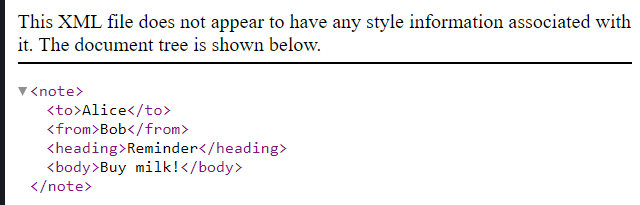
\includegraphics[scale=0.7]{src/XML1.PNG}
\end{center}
Instead, assume now that we had an erroneous XML file, like the one below:
\begin{lstlisting}[language=xml]
<?xml version="1.0" encoding="UTF-8"?>
<note>
    <to>Alice</to>
    <from>Bob</from>
    <heading>Reminder</heading>
    <body>Buy milk!
</note>
\end{lstlisting}
Then, the page will show the error, like shown below:
\begin{center}
    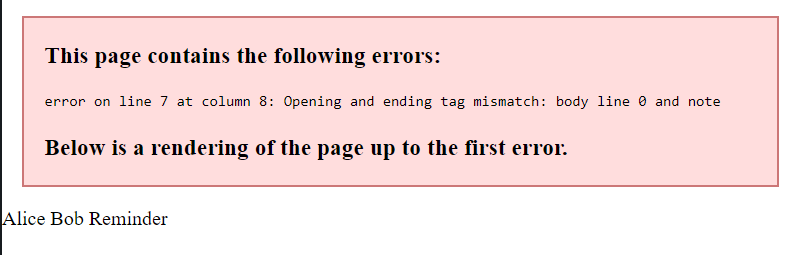
\includegraphics[scale=0.7]{src/XML2.PNG}
\end{center}
There are two ways of using XML in a program. These are:
\begin{itemize}
    \item Using the DOM. This builds an in-memory hierarchical model of the XML elements. It is appropriate if you need the whole document or need to move about it freely.
    \item Using the SAX (the simple API for XML). This provides an event-driven parser for XML. It is appropriate for using parts of the data in the order they appear in the file, or if there are memory constraints.
\end{itemize}

\subsection{DOM Parsing}
DOM is separated into three main parts: the core DOM (the standard model for any structured doc); the HTML DOM (the standard model for HTML docs); and the XML DOM (the standard model for XML docs).

\noindent The XML DOM is a standard object model and programming interface for XML. It defines objects and properties of all XML elements, along with the methods to access them. It is the standard for getting, changing, adding and deleting XML elements. DOM defines everything in an XML document as a node.

\noindent The methods defined on an XML node are the same as those for an HTML node, e.g. \texttt{parentNode}, \texttt{firstChild}, \texttt{nextSibling}, etc.

\noindent When working with an XML file, this is how we want to process it:
\begin{itemize}
    \item Load the XML document object;
    \item Locate the root element or some other element that is of interest- we can either traverse the tree, or search for the desired element;
    \item For the given element, extract the attributes and their values, extract the element data, and/or add, modify or remove elements or attributes;
    \item Restart the cycle until all the processing is complete.
\end{itemize}
The following is an example of DOM parsing in JavaScript:
\begin{lstlisting}[language=javascript]
var text = "<bookstore><book>" + 
    "<title>Everyday Italian</title>" + 
    "<author>Giada De Laurentiis</author>" + 
    "<year>2005</year>" + 
    "</book></bookstore>";
var parser = new DOMParser();

var xmlDoc = parser.parseFromString(text, "text/xml");
var demo = document.getElementById("demo");
demo.innerHTML = xmlDoc.getElementsByTagName("title")[0]
    .childNodes[0].nodeValue;
\end{lstlisting}

\subsection{SAX Parsing}
SAX is a sequential access parser API for XML. It is not an alternative to DOM since there is no default object model, but just another mechanism for reading XML. It is a stream parser that is event-driven. Parsing is unidirectional, i.e. there is no going back. Callback methods are triggered by events when parsing. It is oriented towards state independent processing. An alternative to SAX is StAX, which is oriented to state-dependent processing.

\noindent Events are available for the following XML features:
\begin{itemize}
    \item XML text nodes;
    \item XML element nodes;
    \item XML comments;
    \item XML processing instructions (often used in XPath an XQuery).
\end{itemize}
Events are triggered when open or close element tags are encountered; data (\texttt{\#PCDATA} or \texttt{CDATA}) sections are encountered; or when processing instructions, comments, etc. are encountered.

\noindent There are 3 steps to using SAX in our program:
\begin{itemize}
    \item We create a custom object model, e.g. ResultSet and Result;
    \item We then create a SAX parser;
    \item Finally, we create a DocumentHandler to turn the XML document into instances of our custom object model. The handlers are:
    \begin{itemize}
        \item ContentHandler, which implements the main SAX interface for handling document events;
        \item DTDHandler, which handles DTD events;
        \item EntityResolver, which resolves external entities;
        \item ErrorHandler, which reports errors and warnings; and
        \item DefaultHandler, for everything else.
    \end{itemize}
\end{itemize}

\noindent The following are SAX handler methods:
\begin{itemize}
    \item \texttt{startDocument}, which performs any work required before parsing;
    \item \texttt{endDocument}, which performs any work required at the end of the parsing, e.g. reporting analytical results;
    \item \texttt{startElement(name, attributes)}, which performs any work required when the start tag of an element of that name is encountered;
    \item \texttt{endElement(name)}, which performs any work when the end tag of an element of that name is encountered; and
    \item \texttt{characters(ch)}, which performs any work required when a text node is encountered.
\end{itemize}
We now consider SAX parsing in Java:
\begin{lstlisting}[language=java]
// Employee class (custom object)
public class Employee {
    private int id;
    private String name;
    
    // .. getters, setters and toString
}

// XMLParserSAX class (SAX parser)
public class XMLParserSAX {
    public static void main(String[] args) {
        SAXParserFactory saxParserFactory = SAXParserFactory
            .newInstance();
        try {
            SAXParser saxParser = saxParserFactory.newSAXParser();
            MyHandler handler = new MyHandler();
            saxParser.parse(new File("employees.xml", handler);
        } catch (Exception e) {
            e.printStackTrace();
        }
    }
}

// MyHandler class (handler)
public class MyHandler extends DefaultHandler {
    private List<Employee> empList;
    private Employee emp;
    
    private boolean bAge = false;
    private boolean bName = false;
    private boolean bGender = false;
    private boolean bRole = false;
    
    // initiate the list at the start of the process
    @Override
    public void startDocument() {
        empList = new ArrayList<>();
    }
    
    // at the start of some tag: if tag is employee => make a new 
    // employee with the provided id. If something else is started, 
    // then keep a record of it.
    @Override
    public void startElement(String uri, String localName, 
        String qName, Attributes attributes) throws SAXException {
        if (qName.equalsIgnoreCase("Employee")) {
            emp = new Employee();
            String id = attributes.getValue("id");
            emp.setId(Integer.parseInt(id));
        } else if (qName.equalsIgnoreCase("name")) {
            bName = true;
        } else if (qName.equalsIgnoreCase("age")) {
            bAge = true;
        } else if (qName.equalsIgnoreCase("gender")) {
            bGender = true;
        } else if (qName.equalsIgnoreCase("role")) {
            bRole = true;
        }
    }
    
    // save the text within some tag by finding out the start
    // tag most recently encountered.
    @Override
    public void characters(char ch[], int start, int length) throws 
        SAXException {
        String value = new String(ch, start, length)
        if (bAge) {
            emp.setAge(Integer.parseInt(value));
            bAge = false;
        } else if (bName) {
            emp.setName(value);
            bName = false;
        } else if (bRole) {
            emp.setRole(value);
            bRole = false;
        } else if (bGender) {
            emp.setGender(value);
            bGender = false;
        }
    }
    
    // at the end of the employee tag => save the employee to 
    // the list
    @Override
    public void endElement(String uri, String localName, 
        String qName) throws SAXException {
        if (qName.equalsIgnoreCase("Employee")) {
            empList.add(emp);
        }
    }
    
    // print all the employees
    @Override
    public void endDocument() {
        for (Employee emp: empList) {
            System.out.println(emp);
        }
    }
}
\end{lstlisting}

\noindent In summary, DOM uses more memory and tends to be slower. But, it can handle parsing that requires access to the entire document (if it fits in memory). It is easier to program. Also, it can process files larger than main memory through disk caching. However, this is even slower. On the other hand, SAX uses less memory and tends to be faster. It can also process files that are larger than the main memory. But, it requires more programmer effort. Also, it cannot handle all parsing tasks directly, i.e. if all XML is required for validation.
\newpage

\section{Messages}
Let's look at the 3-tier model again:
\begin{center}
    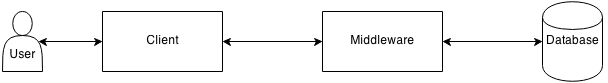
\includegraphics[scale=0.8]{src/L8I1.png}
\end{center}
We have not yet specified how messages are going to be sent, and in what format these messages are going to be. Different interactions will require using different message formats and protocols.

\noindent We shall be focusing on a protocol for communication and the payload formats. HTTP is an application-layer protocol used to send messages. It is a specific URL scheme, and follows a request-response pattern. It provides a number of ways to make a request (i.e. GET and POST). User Agent Specific Protocols (USAP) package and wrap the information that will be sent when providing a response, e.g. XML, XHTML and JSON.

\noindent The request-response pattern is a way to exchange messages. A requester sends a request message, and the receiver of that message provides a message in response. Typically, this is performed in a synchronous fashion (e.g. HTTP), but it can also be asynchronous (e.g. HTTP/2).

\noindent When the user agent (web browser, or client) is asked to send a message, the URL is first turned into an IP address. The request here is asking the Domain Name System (DNS) for the ID. The DNS return the IP for the URL. Secondly, a TCP connection is opened on a particular port on the node at that IP address. Port 80 is the standard port for HTTP, while port 443 is the port for HTTPS, which is encrypted through TLS. Next, a request is made using a specific URL Scheme (e.g. HTTP) and sent using that TCP connection. The request here is to get the home page of the specified URL, while the response is the XHTML for the home page. This can be summarised in the diagram below:
\begin{center}
    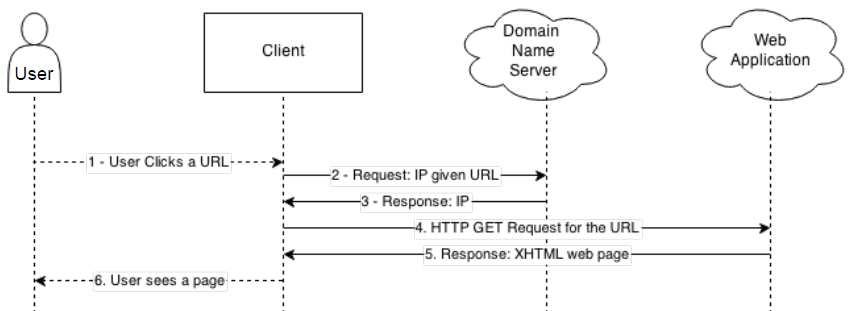
\includegraphics[scale=0.6]{src/L18I1.PNG}
\end{center}
The system architecture design aggregates over all the messages, showing only the flow while hiding a lot of detail. Sequence diagrams provide a better way to show the flow of messages. We label all the messages- the more precise, the better.

\noindent There are other requests, for stylesheets and JavaScript:
\begin{center}
    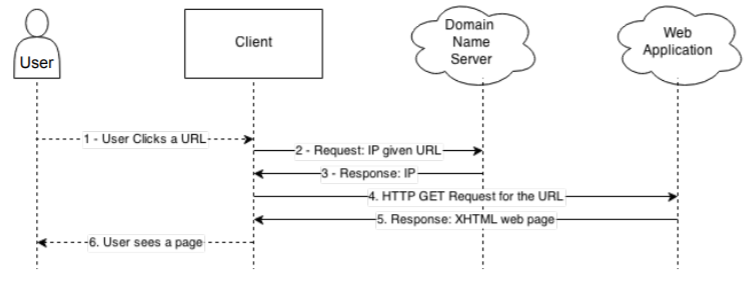
\includegraphics[scale=0.7]{src/L18I2.PNG}
\end{center}
Our web application also communicates with a database. In Django, requests are made indirectly through the Object Relational Mapping (ORM). The actual request maybe via HTTP or some other protocol. But, we can specify it as an ORM request and ORM response.

\noindent Requests can be made using various protocols, such as:
\begin{itemize}
    \item http- this common protocol indicates a file that a web browser can format and display- an HTML file, image file, sound file, etc.
    \item https- this utilises TLS for secure communication, and always sends data in encrypted form.
    \item file- this indicates a file which is not in a recognised web format, and will be displayed as text.
    \item ftp- file transport protocol is used to refer to websites from which files can be extracted and downloaded to client machines.
    \item mailto- if selected, such a link generates a form in which an email message can be constructed and sent to a designated user.
    \item news- the resource is a news group or article.
    \item telnet- it generates a telnet session to this server.
\end{itemize}

\subsection{HTTP}
HyperText Transport Protocol (HTTP) is used to deliver virtually all files and other data using 8-bit characters. Usually, HTTP takes place through TCP/IP sockets. HTTP is used to transmit resources, not just files. A resource is some chunk of information that can be identified by a URI. HTTP functions as a reque-st-response pattern in the client-server computing model.

\noindent Under HTTP, communication is as follows:
\begin{itemize}
    \item An HTTP client opens a connection and sends a request message to an HTTP server. Typically, the request is either a GET or a POST.
    \item The server then returns a response message, usually containing the resource that was request. Typically, this is in XHTML or XML, but it can also be in other formats such as JSON.
    \item After delivering the response, the server closes the connection, making HTTP a stateless protocol. That is, HTTP does not maintain any connection information between transactions.
\end{itemize}
A HTTP get appends the data to the URL as key-value pairs. Special characters within the value are replaced- this is called url encoding. The user can see, copy and bookmark a URL, thus it is easy for them to `resubmit' the page. Therefore, the GET should be used for pages which don't change anything on the server.

\noindent On the other hand, POST sends data packaged as part of the message. It must be used for multipart/form-data, e.g. file uploading. It should be used for programs with side effects, e.g. database update, purchase requested, sending email, etc. It can also be used if there are non-ASCII characters in the data, if the data set is large, or if we want to hide data from users- although they can always view the source. POST uses the message body to acheive this, and so has the following header lines:
\begin{verbatim}
Content-Type: application/x-www-form-urlencoded
Content-Length: 26 // number of characters
\end{verbatim}
and then body, e.g.:
\begin{verbatim}
name=John%20Smith%address=5%20Queen%20Street
\end{verbatim}
We should use GET for safe and idempotent requests, and POST otherwise. A safe operation is an operation which does not change the data requested. An idempotent operation is one in which the result will be the same no matter how many times you request it.

\noindent There are various other HTTP methods, such as:
\begin{itemize}
    \item HEAD, which is like GET but it asks the server to return the response headers only. It is useful to check characteristics of a resource without actually downloading it;
    \item PUT, which is used for storing data on the server;
    \item DELETE, which is used for deleting a resource on the server;
    \item OPTIONS, which is used to find out what the server can do, e.g. switch to secure connections;
    \item TRACE, which is used to debug connections; and
    \item CONNECT, which is used for establishing a link through a proxy.
\end{itemize}
HTTP is a stateless protocol. It does not require the server to retain any information about the client/user- all the requests are independent. This is a problem if we want to maintain a session. There are many common solutions to overcome statelessness:
\begin{itemize}
    \item Client side- we can use HTTP cookies. Cookies are tokens stored on the client and can be included in the request. It is best to store a session id in the cookie that the server can use to retrieve information about the user. We do not store actual data about the user, etc. on their client.
    \item Server side- we can have hidden variables when the page is a form, i.e. through POST methods.
    \item URL encoding- we store a session id within the URL.
\end{itemize}
\newpage

\section{Web-application frameworks}
After developing several web applications (from scratch), it rapidly becomes clear that:
\begin{itemize}
    \item there is a lot of coding overhead and `boiler plate' code;
    \item typically, the same tasks are repeated over and over again, e.g. accessing a database, processing then presenting results in HTML;
    \item There is a need for separation of concerns. Distribution of the main components and interactions to maximise code reuse, provide robustness, aid in debugging, enable scalability, etc.
\end{itemize}
Web frameworks typically provide (some of) the following features:
\begin{itemize}
    \item user authentication, authorisation and security;
    \item database abstraction (or object-relational mapping);
    \item template system;
    \item AJAX sub-framework;
    \item Session management;
    \item An architecture, using based on Model-View-Controller.
\end{itemize}

\subsection{Model-View-Controller}
Model-view-controller is a design pattern. A design pattern serves as a tool to communicate ideas, solutions and knowledge about commonly recurring design problems. User interface design patterns help designers and developers create the most effective and usable interface for a particular situation. Thus, each pattern is a three-part rule, which expresses a relation between a certain context, a problem, and a solution. Patterns can be expressed hierarchically, with each layer representing a different level of granularity. There may also be many different ways to (physically) implement each pattern.

\noindent When using GUIs, we want to separate the concerns between the presentation logic, business and application logic and the data model. The architecture pattern Model View Controller was developed for this. It maps the traditional input, processing, output roles into the GUI realm.

\noindent The controller interprets the mouse and keyboard inputs, and maps these to actions. These commands are sent to the model or view to enact the appropriate change. The model manages the data elements- it responds to queries about its state, and updating it. The view manages the display for presenting the data.

\noindent In more detail, the three parts do the following:
\begin{itemize}
    \item The model contains code that operates on the application data. Any actions wanted to be executed on the raw data must go through this layer. Definitions of how the application works with data (commonly CRUD: create, read, update or delete) are written here.
    \item The view is the presentation layer. It defines how the pages should look to the user, how the application presents data, or how a user can submit certain instructions to be executed by the application.
    \item The controller acts as the orchestrator of the application. It controls the flow of the program. It receives user commands, processes them and then contacts the model, and finally instructs the view to display appropriately to the user.
\end{itemize}
The models represent application data and the domain logic. It notifies the views when it changes, and enables the view to query the model. It allows the controller to access application data functionality enapsulated by the model.

\noindent A view is a (visual) representation of its model and acts as a presentation filter. It renders the contents of the model, and specifies how the model data should be presented. A view is attached to its model (or model part), and gets the data necessary for the presentation from the model by asking questions. So, when the model changes, the view must update its presentation. We can have a push model- the view registers itself with the model for change notifications, or a pull model- the view is representation for calling the model when it needs to retrieve the most current data. The view is responsible for forwarding user request/gestures to the controller.

\noindent The controller defines the application behaviour. A controller is the link between a user and the system. It interprets user requests/gestures and map them into actions for the model to perform. It arranges for relevant views to present themselves in appropriate places on the screen.

\noindent The following image summarises the interaction between the model, the view and the controller:
\begin{center}
    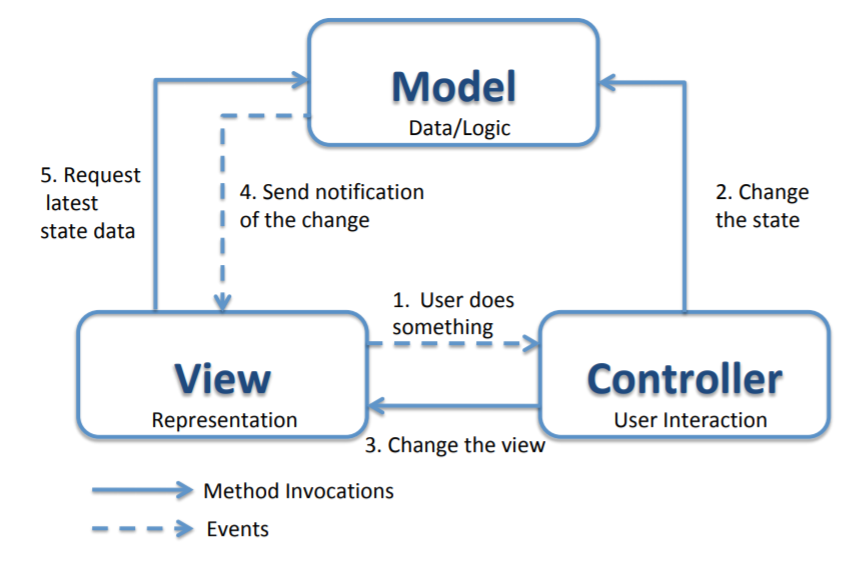
\includegraphics[scale=0.5]{src/L19I1.PNG}
\end{center}
There are many advantages to the MVC. It enables independent development and testing. It is easier to maintain. It provides reusable views and models. We can synchronise views and have multiple simultaneous views. It helps enforce logical separation of concerns. 

\noindent However, the MVC also has some disadvantages. There are some initial overheads splitting up concerns. We have increased overheads in development (i.e. 3 classes, not 1), especially for very simple applications. Debugging can sometimes be a problem. It requires the developers to understand patterns.

\noindent In Django, MVC can be a bit confusing. The `views' receive input, query and process data, and might be considered part of the controller role in traditional MVC. We often say MVCT (model, view, controller, template) or just MTV rather than MVC. Here, the 3 aspects are:
\begin{itemize}
    \item The models describe the database;
    \item The controller is handled by the Django framework, and the URL parser. The URL parser maps urls to views, where processing may occur.
    \item The templates describe how the data is presented.
\end{itemize}

\subsection{Frameworks}
As with real world frameworks, software frameworks provide design and partial implementation for a particular domain of applications. Frameworks allow developers to create applications more efficiently by providing default functionality, whilst allowing them to extend and override to suit their specific purposes.

\noindent There are several interpretations of a framework:
\begin{itemize}
    \item A framework is a set of classes that embodies an abstract design for solutions to a family of problems;
    \item A framework is a set of prefabricated software building blocks that programmers can use, extend or customise for specific computing solutions;
    \item Frameworks are large abstract applications in a particular domain that can be tailored for individual applications;
    \item A framework is a reusable software architecture comprising both design and code.
\end{itemize}
Virtually all web applications have a common set of basic requirements, such as user management, security, password recovery, sessions management, database management, etc. Frameworks encapsulate thousands of hours of experience, knowledge and know-how. It improves over each iteration, is debugged and secure. It can often handle reasonably high loads and traffic out of the box.

\noindent Below are some characteristics of a framework:
\begin{itemize}
    \item Inversion of control- the framework is responsible for the application control flow;
    \item Default behaviour- framework must provide some `useful' functionality related to the application domain;
    \item Extensibility- hotspots within the framework are designed to be extended. It allows a developer to customise their application specifically for a particular response;
    \item Non-modifiable framework code: key components of the framework cannot be altered. It may not be strictly non-modifiable, but typically just used, though contributions back to the framework are often subject to the framework creators or open source company.
\end{itemize}
There are many advantages to using a framework. It enables rapid development since we can concentrate on unique application logic. It reduces boilerplate code. It is already built and tested, so we have increased reliability. In general, there is increased security. There is a high level of support for basic common functionality.

\noindent However, there are also some disadvantages. It imposes a certain model of development (80\% easy, 20\% hard). Frameworks can introduce code bloat. The levels of abstraction generally introduce performance penalties. It is difficult to overcome the steep learning curve. The framework may be poorly documented. A bug or security risk in the framework can seriously compromise the application.

\noindent A framework is about reusing behaviours by controlling how abstract classes and components interact with each other. A framework will call our application code. On the other hand, a library is a collection of classes which provide reusable functionality. Our application will call the library.

\noindent Most frameworks have the following:
\begin{itemize}
    \item Web template system, to provide pre-defined pages that load dynamic content;
    \item Caching, to reduce perceived lag;
    \item Security, to provide authentication and authorisation functionality;
    \item Database access and mapping, to speed up working with databases and avoid using SQL.
    \item URL mapping, to enable handling of URLs and friendlier URls;
    \item AJAX handlers and handling, to create more dynamic pages that are more responsive;
    \item Automatic configuration, to decrease the setup hassles, usually using introspection and/or following conventions;
    \item Form management, to speed up the creation of forms and handling of forms.
\end{itemize}
We use web-app frameworks to reduce `boiler plate' code in web applications. This helps particular with accessing and manipulating the database. It is often reffered to as CRUD operations. We also have session management across multiple pages. Web apps have matured to a point where software engineering practices (including design patterns and frameworks) are becoming increasingly useful, necessary and the norm.

\noindent Nonetheless, they require an investment in learning the framework. There is a trade off between learning the framework and building it ourselves. We also sacrifice some flexibility for rapid development. There is another trade off between flexibility and efficiency here. Like client-side libraries, knowledge of one framework does not necessarily transform to another. We are in the early stages of web framework ecosystem. There are many competing options at present. Eventually, the most popular (few) will emerge.

\end{document}